\documentclass[a4paper,twoside]{book}

\emergencystretch=1em
\usepackage[utf8]{inputenc}
\usepackage[english,russian]{babel}
\usepackage{fontspec}
\usepackage{graphicx}
\renewcommand{\thefigure}{\thesection.\arabic{figure}}
\usepackage{hyperref}
\usepackage{multirow}
\usepackage[absolute,overlay,showboxes]{textpos}
\usepackage{etoolbox}
\usepackage{longtable}
\usepackage{tikz}
\usepackage{lilyglyphs}
\usepackage{tabularx}
\usepackage{pgfplots}
\usepackage{circuitikz}
\usepackage{glossaries}
\usepackage{makeidx}
\usepackage{expl3}
\usepackage{chngcntr}
\usepackage{svg}
\usepackage{subfiles}
\usepackage[printonlyused,withpage]{acronym}

\usepackage[backend=bibtex]{biblatex}
\addbibresource{references.bib}

%%%%%%%%%%%%%%%%%%%%%%%%%%%%%%%%%%%%%%%%%%%%%%%%%%%%%%%%%%%%%%%%%%%%%%%%%%%%%%%%
%% Set the Minted style.

\definecolor{friendlybg}{HTML}{f0f0f0}
\setminted[cpp]
          {
            style=friendly,
            bgcolor=friendlybg,
            linenos
          }

\newbool{oldminted}

\newread\mypipe
\openin\mypipe="|kpsewhich minted2.sty"
\ifeof\mypipe
\else
\begingroup
\endlinechar=-1
\read\mypipe to \x
\ifdefempty{\x}{
  \global\booltrue{oldminted}
}{
  \global\boolfalse{oldminted}
}
\endgroup
\fi

\ifbool{oldminted} {
  \usepackage{minted}
} {
  \usepackage{minted2}
}

\definecolor{friendlybg}{HTML}{f0f0f0}
\setminted[cpp]
          {
            fontsize=\small,
            style=friendly,
            bgcolor=friendlybg,
            linenos
          }
          %%


%%%%%%%%%%%%%%%%%%%%%%%%%%%%%%%%%%%%%%%%%%%%%%%%%%%%%%%%%%%%%%%%%%%%%%%%%%%%%%%%
\setmainfont{Liberation Serif}
\setmonofont{Liberation Mono}

\makeindex
\makeglossaries

\urlstyle{same}

\graphicspath{ {images/} {../../../images/} {../../../out/src/common/} }

%% \documentclass[../main.tex]{subfiles}
%% \usepackage{svg}
%% \graphicspath{{\subfix{../images/}}}
%% \begin{document}

\newcounter{example-counter}
\setcounter{example-counter}{1}

%% This procedure adds the "Example" block to the text.
\newcommand{\example}[1]{
  \vspace{8pt}
  \begin{tabularx}{\textwidth}{m{1cm} m{9cm}}
    \includesvg[width=1.25cm]{the-noun-project/request-mirrored}
    & \textbf{Пример \arabic{example-counter}}: #1 \\
  \end{tabularx}
  \addtocounter{example-counter}{1}
}

\newcounter{experiment-counter}
\setcounter{experiment-counter}{1}

%% This procedure adds the "Experiment" block to the text.
\newcommand{\experiment}[2]{
  \vspace{8pt}
  \begin{tabularx}{\textwidth}{m{.15\textwidth}X m{.85\textwidth-4}X}
    \includesvg[width=1cm]{the-noun-project/flask}
    & \textbf{Эксперимент №\arabic{experiment-counter}:} #2 \\
  \end{tabularx}
  \addtocounter{experiment-counter}{1}
}

\newcommand{\note}[1]{
  \vspace{8pt}
  \begin{tabularx}{\textwidth}{m{1cm} m{9cm}}
    \includesvg[width=1cm]{the-noun-project/note}
    & \textbf{Примечание:} #1 \\
  \end{tabularx}
}

\newcommand{\hotkey}[1]{
  \texttt{#1}
}

%% This procedure allows to insert a music note.
%% Syntax:
%%   \musicnote{<octave>}{<note-name>}{<frequency>}
\newcommand{\musicnote}[3]{
  &
  \ifstrequal{#2}{C}{До   & C#1}{}
  \ifstrequal{#2}{D}{Ре   & D#1}{}
  \ifstrequal{#2}{E}{Ми   & E#1}{}
  \ifstrequal{#2}{F}{Фа   & F#1}{}
  \ifstrequal{#2}{G}{Соль & G#1}{}
  \ifstrequal{#2}{A}{Ля   & A#1}{}
  \ifstrequal{#2}{B}{Си   & B#1 (H#1)}{}
  & #3 \\
}

%% Taken from:
%%   <https://tex.stackexchange.com/questions/184923/how-to-include-a-second-file-only-if-environment-variable-is-set>
\newcommand{\newgetenv}[2][]{%
 \CatchFileEdef{\temp}{"|kpsewhich --var-value #2"}{\endlinechar=-1\relax}%
 \if\relax\detokenize{#1}\relax\temp\else\edef#1{\temp}\fi%
}%

\newcommand\esymbol[1]{%
  \begin{circuitikz}%
    \draw (0,0) to [#1] (1,0);%
  \end{circuitikz}%
}

\newcommand*{\soundWaveIcon}[0]{%
  \begin{tikzpicture}
    \draw[black, fill=black] (0, 0) circle (.25mm);
    \draw (.5mm, 0.7mm) arc (45:-45:1mm);
    \draw (1mm, 1mm) arc (45:-45:1.5mm);
    \draw (1.5mm, 1.3mm) arc (45:-45:2mm);
  \end{tikzpicture}%
}

%% \end{document}


\newcommand{\figureADC}[1]{
  \def\lang{\detokenize{#1}}
  \def\langRu{\detokenize{ru}}
  \def\langEn{en}
  \def\figureCaption{XXX: No translation.}
  \ifx \lang\langRu
  \def\figureCaption{
    Схематическое изображение 10-битного аналогово-цифрового
    преобразователя (АЦП.)
  }
  \fi
  \if \lang\langEn
  \def\figureCaption{
    Schematic depiction of the 10-bit analog-to-digital converted (ADC.)
  }
  \fi
  \begin{figure}[ht]
    \centering
    \begin{tikzpicture}
      \draw[thick] (0, 0) -- (0, 5.5) -- (3, 5.5) -- (3, 0) -- (0, 0);
      \draw (1.5, 2.5) node[right, above] {ADC};
      \draw (1.5, 5.5) -- (1.5, 6.5) node[right, above] {VCC};
      \draw (1.5, 0) -- (1.5, -1) node[right, below] {GND};
      \draw (-2, 5.0)
      -- (-1, 5.0) node[left, above, text width=2cm] {$V_{ref}$}
      -- (0, 5.0);
      \draw (0, 3.00)
      -- (-1, 3.00) node[left, above, text width=2cm] {ANALOG INPUT}
      -- (-2, 3.00);
      \draw (-2, 0.5)
      -- (-1, 0.5) node[left, above, text width=2cm] {CLOCK INPUT}
      -- (0, 0.5);
      \draw(-0.25, 0.25) -- (0.25, 0.75);
      \foreach \n/\y in {0/0.5, 1/1.0, 2/1.5, 3/2.0, 4/2.5, 5/3.0, 6/3.5, 7/4.0, 8/4.5, 9/5.0} {
        \draw (3, \y) node[anchor=south west] {OUTPUT \n} -- (5, \y);
      };
    \end{tikzpicture}
    \caption{\figureCaption}
    \label{fig:adc-schematics}
  \end{figure}
}

\newcommand{\figureAVRMemory}[1]{
  \def\lang{\detokenize{#1}}
  \def\langRu{\detokenize{ru}}
  \def\langEn{\detokenize{en}}
  \def\figureCaption{XXX: No translation.}
  \ifx \lang\langRu
  \def\figureCaption{
    Карта памяти AVR.
  }
  \fi
  \ifx \lang\langEn
  \def\figureCaption{
    AVR memory map.
  }
  \fi
  \begin{figure}[H]
    \centering
    \begin{tikzpicture}
      \path[shape=coordinate]
      (0,5) coordinate(b1) (2,5) coordinate(b2)
      (2,2) coordinate(b3) (0,2) coordinate(b4);
      \filldraw[fill=white!80!black] (b1) -- (b2) -- (b3) -- (b4) -- (b1);
      \draw (1, 3.5) node[anchor=south] {Flash};
      \draw (b2) node[anchor=west] {\small{0x0000}};

      \path[shape=coordinate]
      (0,0) coordinate(b5) (2,0) coordinate(b6);
      \filldraw[fill=white!80!black] (b3) -- (b4) -- (b5) -- (b6) -- (b3);
      \draw (1, 1.5) node[anchor=south] {Boot section};
      \draw (b6) node[anchor=south west] {\small{F\_END}};

      \path[shape=coordinate]
      (4,5) coordinate(b7) (6,5) coordinate(b8)
      (6,3) coordinate(b9) (4,3) coordinate(b10);
      \filldraw[fill=white!80!black] (b7) -- (b8) -- (b9) -- (b10) -- (b7);
      \draw (5, 4) node[anchor=center] {
        \shortstack{32 general \\  purpose \\ registers}
      };
      \draw (b8) node[anchor=west] {\small{0x0000}};
      \draw (b9) node[anchor=south west] {\small{0x001F}};

      \path[shape=coordinate]
      (4,3) coordinate(b11) (6,3) coordinate(b12)
      (6,1) coordinate(b13) (4,1) coordinate(b14);
      \filldraw[fill=white!80!black] (b11) -- (b12) -- (b13) -- (b14) -- (b11);
      \draw (5, 2) node[anchor=center] {
        \shortstack{64 I/O \\ registers}
      };
      \draw (b12) node[anchor=north west] {\small{0x0020}};
      \draw (b13) node[anchor=south west] {\small{0x005F}};
      \draw (b13) node[anchor=north west] {\small{0x0060}};

      \path[shape=coordinate]
      (4,1) coordinate(b14) (6,1) coordinate(b15)
      (6,-1) coordinate(b16) (4,-1) coordinate(b17);
      \filldraw[fill=white!80!black] (b14) -- (b15) -- (b16) -- (b17) -- (b14);
      \draw (5, 0) node[anchor=center] {
        \shortstack{Additional \\ I/O \\ registers}
      };

      \path[shape=coordinate]
      (4,-1) coordinate(b18) (6,-1) coordinate(b19)
      (6,-2) coordinate(b20) (4,-2) coordinate(b21);
      \filldraw[fill=white!80!black] (b18) -- (b19) -- (b20) -- (b21) -- (b18);
      \draw (5, -1.5) node[anchor=center] {
        \shortstack{Internal \\ RAM}
      };
      \draw (b20) node[anchor=south west] {\small{RAM\_END}};
      \draw (b20) node[anchor=north west] {\small{RAM\_END + 1}};

      \path[shape=coordinate]
      (4,-2) coordinate(b22) (6,-2) coordinate(b23)
      (6,-3) coordinate(b24) (4,-3) coordinate(b25);
      \filldraw[fill=white!80!black] (b22) -- (b23) -- (b24) -- (b25) -- (b22);
      \draw (5, -2.5) node[anchor=center] {
        \shortstack{External \\ RAM}
      };
      \draw (b24) node[anchor=south west] {\small{0xFFFF}};

      \path[shape=coordinate]
      (8,5) coordinate(b26) (10,5) coordinate(b27)
      (10,3) coordinate(b28) (8,3) coordinate(b29);
      \filldraw[fill=white!80!black] (b26) -- (b27) -- (b28) -- (b29) -- (b26);
      \draw (9, 4) node[anchor=center] {
        \shortstack{EEPROM}
      };
      \draw (b27) node[anchor=west] {\small{0x0000}};
      \draw (b28) node[anchor=south west] {\small{E\_END}};
    \end{tikzpicture}
    \caption{\figureCaption}
    \label{fig:avr-memory}
  \end{figure}
}

\newcommand{\figureAnalogSignalExample}[1]{
  \begin{figure}[ht]
    \begin{tikzpicture}
      \draw[thick, ->] (0, 0) -- (12, 0) node[anchor=north west] {t};
      \draw[thick, ->] (0, 0) -- (0,  7) node[anchor=south west] {V};
      \draw[gray] (0, 0) grid (10, 6);
      \draw[ultra thick, red] (0,1)   sin (1,4);
      \draw[ultra thick, red] (1,4)   cos (2,2);
      \draw[ultra thick, red] (2,2)   sin (3,0.5);
      \draw[ultra thick, red] (3,0.5) cos (4,2);
      \draw[ultra thick, red] (4,2)   sin (4.5,3);
      \draw[ultra thick, red] (4.5,3) cos (5,2);
      \draw[ultra thick, red] (5,2)   sin (5.5,1);
      \draw[ultra thick, red] (5.5,1) cos (6.5,4);
      \draw[ultra thick, red] (6.5,4) sin (7,5);
      \draw[ultra thick, red] (7,5)   cos (8,2);
      \draw[ultra thick, red] (8,2)   sin (8.5,1);
      \draw[ultra thick, red] (8.5,1) cos (10, 3);
    \end{tikzpicture}
    \caption{#1}
    \label{fig:adc-analog-signal-example}
  \end{figure}
}

\newcommand{\figureArray}[1]{
  \def\lang{\detokenize{#1}}
  \def\langRu{\detokenize{ru}}
  \def\langEn{\detokenize{en}}
  \def\figureCaption{XXX: No translation.}
  \ifx \lang\langRu
  \def\figureCaption{
    Схематическое изображение массива 4x20 (4 строки, 20 столбцов.)
  }
  \fi
  \ifx \lang\langEn
  \def\figureCaption{
    A schematic representation of a 2-dimensional array 4x20 (4 rows, 20
    columns.)
  }
  \fi
  \begin{figure}[ht]
    \centering
    \begin{tikzpicture}
      \draw[step=0.5cm,black,very thin] (-5, -2) grid (5, 0);
      \foreach[count=\n from 0] \x in {-5, -4.5, ..., 4.5} {
        \draw (\x cm, 0) node[anchor=south west] {$\n$};
      }
      \foreach[count=\n from 0] \y in {-0.5, -1.0, ..., -2} {
        \draw (-5.5, \y) node[anchor=south west] {$\n$};
      }
    \end{tikzpicture}
    \caption{\figureCaption}
    \label{fig:2d-array-example}
  \end{figure}
}

\newcommand{\figureArrayOfPointers}[1]{
  \def\lang{\detokenize{#1}}
  \def\langRu{\detokenize{ru}}
  \def\langEn{\detokenize{en}}
  \def\figureCaption{XXX: No translation.}
  \ifx \lang\langRu
  \def\figureCaption{
    Схематическое представление массива 4x20 в виде одномерного массива из 4-х
    элементов со ссылками на одномерные массивы по 20 элементов.
  }
  \fi
  \ifx \lang\langEn
  \def\figureCaption{
    A schematic representation of an 4x20 array as a one-dimensional array of 4
    elements that hold pointers to one-dimensional arrays of 20 elements.
  }
  \fi
  \begin{figure}[H]
    \centering
    \begin{tikzpicture}
      \draw[step=0.5cm,black,very thin] (-5, -2) grid (-4.5, 0);
      \draw[step=0.5cm,black,very thin] (-4, -2) grid (6, 0);
      \foreach[count=\n from 0] \x in {-4, -3.5, ..., 5.5} {
        \draw (\x cm, 0) node[anchor=south west] {$\n$};
      }
      \foreach[count=\n from 0] \y in {-0.5, -1.0, ..., -2} {
        \draw (-5.5, \y) node[anchor=south west] {$\n$};
      }
      \foreach[count=\n from 0] \y in {-0.25, -0.75, ..., -2} {
        \draw[{Circle}-{Stealth}]  (-4.8, \y) -- (-4, \y);
      }
    \end{tikzpicture}
    \caption{\figureCaption}
    \label{fig:2d-array-example-with-references}
  \end{figure}
}

\newcommand{\figureBigLCD}[1]{
  \def\lang{\detokenize{#1}}
  \def\langRu{\detokenize{ru}}
  \def\langEn{\detokenize{en}}
  \def\figureCaption{XXX: No translation.}
  \ifx \lang\langRu
  \def\figureCaption{
    Схематическое изображение внешнего вида ЖК-дисплея 20x4 (источник
    изображения:
    \url{https://commons.wikimedia.org/wiki/File:LCD_20x4_breadboard.svg}.)
  }
  \fi
  \ifx \lang\langEn
  \def\figureCaption{
    A schematic representation of the outer appearance of an 20x4 LCD (image
    source:
    \url{https://commons.wikimedia.org/wiki/File:LCD_20x4_breadboard.svg}.)
  }
  \fi
  \begin{figure}[h]
    \centering
    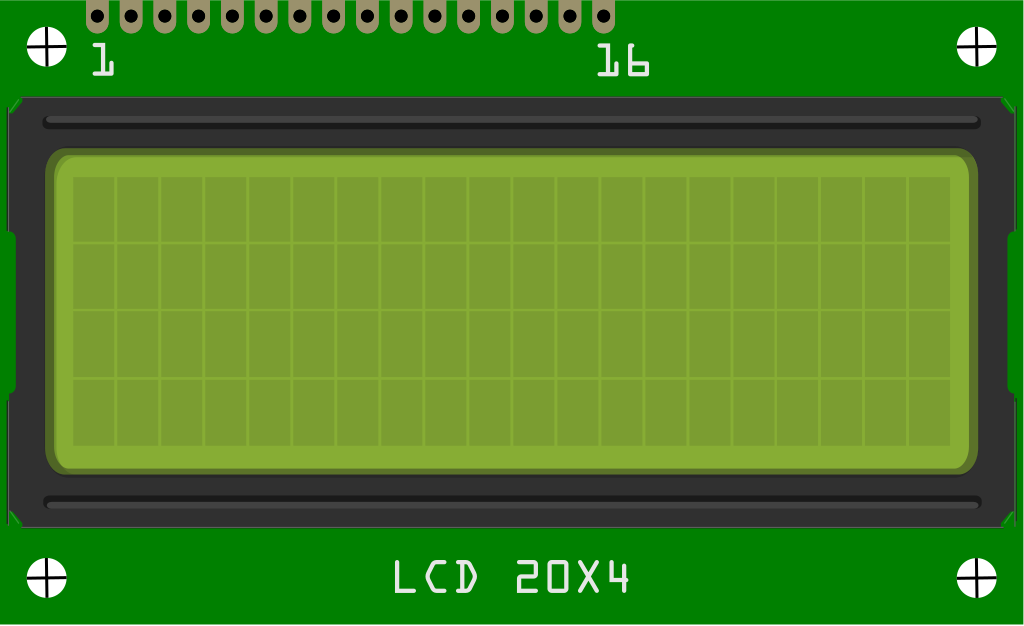
\includegraphics[width=10cm]{lcd-20x4}
    \caption{\figureCaption}
    \label{fig:lcd-20x4}
  \end{figure}
}

\newcommand{\figureBigLCDShematics}[1]{
  \def\lang{\detokenize{#1}}
  \def\langRu{\detokenize{ru}}
  \def\langEn{\detokenize{en}}
  \def\figureCaption{XXX: No translation.}
  \ifx \lang\langRu
  \def\figureCaption{
    Схематическое изображение дисплея 20x4 (20 столбцов, 4 строки.)
  }
  \fi
  \ifx \lang\langEn
  \def\figureCaption{
    A schematic representation of an 20x4 LCD (20 columns, 4 rows.)
  }
  \fi
  \begin{figure}[ht]
    \centering
    \begin{tikzpicture}
      \draw[gray, step=0.5] (0, 0) grid (10, 2);
      \foreach [count=\i from 0] \x in {0.0, 0.5, 1.0, ..., 9.5} {
        \draw (\x, 2.5) node[anchor=north west] {\i};
      }
      \foreach [count=\i from 0] \y in {1.5, 1.0, ..., 0.0} {
        \draw (-0.5, \y) node[anchor=south west] {\i};
      }
    \end{tikzpicture}
    \caption{\figureCaption}
    \label{fig:lcd-20x4-schematics}
  \end{figure}
}

\newcommand{\figureBlinkinLEDGraph}[1]{
  \def\lang{\detokenize{#1}}
  \def\langRu{\detokenize{ru}}
  \def\langEn{en}
  \def\figureCaption{XXX: No translation.}
  \ifx \lang\langRu
  \def\figureCaption{
    Графическое отображение сигнала, меняющегося во времени, на цифровом
    порту.
  }
  \fi
  \if \lang\langEn
  \def\figureCaption{
    Graphical representation of a signal in relation to the time on a
    digital port.
  }
  \fi
  \begin{figure}[ht]
    \begin{tikzpicture}
      \draw[thick, ->] (0, 0) -- (12, 0) node[anchor=north west] {t};
      \draw[thick, ->] (0, 0) -- (0,  7) node[anchor=south west] {V};
      \draw[lightgray] (0, 0) grid (10, 6);
      \foreach \x in {0, 2, ..., 8} {
        \draw[ultra thick, teal] (\x, 6) -- (\x + 1, 6);
        \draw[ultra thick, teal] (\x + 1, 6) -- (\x + 1, 1);
        \draw[ultra thick, teal] (\x + 1, 1) -- (\x + 2, 1);
        \draw[ultra thick, teal] (\x + 2, 1) -- (\x + 2, 6);
      }
    \end{tikzpicture}
    \caption{\figureCaption}
    \label{fig:blinking-led-graph}
  \end{figure}
}

\newcommand{\figureButtonBounceGraph}[1]{
  \def\lang{\detokenize{#1}}
  \def\langRu{\detokenize{ru}}
  \def\langEn{\detokenize{en}}
  \def\figureCaption{XXX: No translation.}
  %% \def\figureUnit{$\mu\mbox{s}$}
  \ifx \lang\langRu
  \def\figureCaption{
    Эффект ``дребезга'' контактов.
  }
  \fi
  \ifx \lang\langEn
  \def\figureCaption{
    Button bounce effect.
  }
  \fi
  \begin{figure}[H]
    \begin{tikzpicture}[samples=200, domain=0:5*360]
      \draw[lightgray] (0, 0) grid (10, 6);
      \draw[thick, orange] (0,  1) -- (4,   1);
      \foreach \x in {4.0, 4.5, 5.0} {
        \pgfmathsetmacro{\mx}{\x + 0.25 + random(0,2) / 8}
        \pgfmathsetmacro{\my}{5 - random(0,4) / \x}
        \pgfmathsetmacro{\ex}{\x + 0.5}
        \draw[thick, orange] (\x,  1)
        -- (\mx, \my)
        -- (\ex, 1);
      };
      \draw[thick, orange] (5.5, 1) -- (6,  5) -- (10, 5);
      \draw[thick, ->] (0, 0) -- (11, 0) node[anchor=north west] {t};
      \draw[thick, ->] (0, 0) -- (0,  7) node[anchor=south west] {V};
    \end{tikzpicture}
    \caption{\figureCaption}
    \label{fig:button-bounce-graph}
  \end{figure}
}

\newcommand{\figureButtonCircuit}[1]{
  \def\lang{\detokenize{#1}}
  \def\langRu{\detokenize{ru}}
  \def\langEn{\detokenize{en}}
  \def\figureCaption{XXX: No translation.}
  \def\figureButtonTitle{XXX: No translation.}
  \ifx \lang\langRu
  \def\figureCaption{
    Возможная схема подключения кнопки к Arduino.
  }
  \def\figureButtonTitle{
    Тактовая кнопка.
  }
  \fi
  \ifx \lang\langEn
  \def\figureCaption{
    One of the possible ways to connect a button to an Arduino.
  }
  \def\figureButtonTitle{
    A push button.
  }
  \fi
  \begin{figure}[H]
    \centering
    \begin{circuitikz}
      \draw (3.5, 0) node[
        dipchip,
        num pins=2,
        external pins width=0.0,
        no topmark,
        hide numbers,
        xscale = 2.5,
        yscale = 2.5](C1){Arduino};
      \node [above left, font=\small] at (C1.bpin 1) {5V};
      \node [above right, font=\small] at (C1.bpin 2) {2};
      \draw
      (C1.bpin 1) to[short]
      (0, 0) to[short]
      (0, 4) to[push button, l=\figureButtonTitle] (7, 4)
      (7, 4) to[short]
      (7, 0) to[short]
      (C1.bpin 2);
    \end{circuitikz}
    \caption{\figureCaption}
    \label{fig:game-dev-button-00}
  \end{figure}
}

\newcommand{\figureButtonPulldownResistorCircuit}[1]{
  \def\lang{\detokenize{#1}}
  \def\langRu{\detokenize{ru}}
  \def\langEn{\detokenize{en}}
  \def\figureCaption{XXX: No translation.}
  \def\figureButtonTitle{XXX: No translation.}
  \ifx \lang\langRu
  \def\figureCaption{
    Схема подключения кнопки к Arduino с подтягивающим резистором.
  }
  \def\figureButtonTitle{
    Тактовая кнопка.
  }
  \fi
  \ifx \lang\langEn
  \def\figureCaption{
    One of the possible ways to connect a button with a pull-down resistor an
    Arduino.
  }
  \def\figureButtonTitle{
    A push button.
  }
  \fi
  \begin{figure}[H]
    \centering
    \begin{circuitikz}
      \draw (3.5, 0) node[
        dipchip,
        num pins=3,
        external pins width=0.0,
        no topmark,
        hide numbers,
        xscale = 2.5,
        yscale = 2.5](C1){Arduino};
      \node [above left, font=\small] at (C1.bpin 1) {5V};
      \node [above right, font=\small] at (C1.bpin 2) {2};
      \node [above right, font=\small] at (C1.bpin 3) {GND};
      \draw
      (C1.bpin 1) to[short]
      (0, 0.35) to[short]
      (0, 4) to[push button, l=\figureButtonTitle] (9, 4)
      (9, 4) to[short]
      (9, -0.35) to[short]
      (C1.bpin 2);
      \draw
      (C1.bpin 3) to [short]
      (7, 1) to [european resistor, l=$R_1$]
      (8, 1) to [short]
      (9, 1);
    \end{circuitikz}
    \caption{\figureCaption}
    \label{fig:game-dev-button-with-pull-down-resistor}
  \end{figure}
}

\newcommand{\figureButtonPullupResistorCircuit}[1]{
  \def\lang{\detokenize{#1}}
  \def\langRu{\detokenize{ru}}
  \def\langEn{\detokenize{en}}
  \def\figureCaption{XXX: No translation.}
  \def\figureButtonTitle{XXX: No translation.}
  \ifx \lang\langRu
  \def\figureCaption{
    Схема подключения кнопки к Arduino при использовании встроенного
    подтягивающего резистора к 5V.
  }
  \def\figureButtonTitle{
    Тактовая кнопка.
  }
  \fi
  \ifx \lang\langEn
  \def\figureCaption{
    One of the possible ways to connect a button using an embedded pull-down
    resistor to an Arduino.
  }
  \def\figureButtonTitle{
    A push button.
  }
  \fi
  \begin{figure}[H]
    \centering
    \begin{circuitikz}
      \draw (3.5, 0) node[
        dipchip,
        num pins=2,
        external pins width=0.0,
        no topmark,
        hide numbers,
        xscale = 2.5,
        yscale = 2.5](C1){Arduino};
      \node [above left, font=\small] at (C1.bpin 1) {GND};
      \node [above right, font=\small] at (C1.bpin 2) {2};
      \draw
      (C1.bpin 1) to[short]
      (0, 0) to[short]
      (0, 4) to[push button, l=\figureButtonTitle] (7, 4)
      (7, 4) to[short]
      (7, 0) to[short]
      (C1.bpin 2);
    \end{circuitikz}
    \caption{\figureCaption}
    \label{fig:game-dev-button-with-pull-up-resistor}
  \end{figure}
}

\newcommand{\figureDigitalSignalExample}[1]{
  \begin{figure}[ht]
    \begin{tikzpicture}
      \draw[thick, ->] (0, 0) -- (12, 0) node[anchor=north west] {t};
      \draw[thick, ->] (0, 0) -- (0,  7) node[anchor=south west] {V};
      \draw[gray] (0, 0) grid (10, 6);
      \foreach \x in {0, 2, ..., 8} {
        \draw[ultra thick, red] (\x, 6) -- (\x + 1, 6);
        \draw[ultra thick, red] (\x + 1, 6) -- (\x + 1, 1);
        \draw[ultra thick, red] (\x + 1, 1) -- (\x + 2, 1);
        \draw[ultra thick, red] (\x + 2, 1) -- (\x + 2, 6);
      }
    \end{tikzpicture}
    \caption{#1}
    \label{fig:adc-digital-signal-example}
  \end{figure}
}

\newcommand{\figureElectronicsResistance}[1]{
  \def\lang{\detokenize{#1}}
  \def\langRu{\detokenize{ru}}
  \def\langEn{\detokenize{en}}
  \def\figureCaption{XXX: No translation.}
  \ifx \lang\langRu
  \def\figureCaption{
    Пример ёмкостей, соединённых трубами разных сопротивлений.
  }
  \fi
  \ifx \lang\langEn
  \def\figureCaption{
    An example of two vessels connected with pipes with different resistance to
    the water flow.
  }
  \fi
  \begin{figure}[ht]
    \centering
    \def\offset{6}
    \begin{tikzpicture}[
        declare function={f1(\x) = 0.15 * sin(8.0 * deg(\x));
      }]

      \draw[thick] (0, 0) -- (0, 4);
      \draw[thick] (2, 0.5) -- (2, 4);
      \draw[thick] (0, 0) -- (2, 0);

      \draw[thick] (3, 0.5) -- (3, 4);
      \draw[thick] (5, 0) -- (5, 4);
      \draw[thick] (3, 0) -- (5, 0);

      \draw[thick] (2, 0) -- (3, 0);
      \draw[thick] (2, 0.5) -- (3, 0.5);

      \draw[thick] (\offset, 0) -- (\offset, 4);
      \draw[thick] (\offset + 2, 0.25) -- (\offset + 2, 4);
      \draw[thick] (\offset, 0) -- (\offset + 2, 0);

      \draw[thick] (\offset + 3, 0.25) -- (\offset + 3, 4);
      \draw[thick] (\offset + 5, 0) -- (\offset + 5, 4);
      \draw[thick] (\offset + 3, 0) -- (\offset + 5, 0);

      \draw[thick] (\offset + 2, 0) -- (\offset + 3, 0);
      \draw[thick] (\offset + 2, 0.25) -- (\offset + 3, 0.25);

      \draw[thick, color=red, ->] (2.5, 1.5) -- (2.5, 0.5);
      \draw[thick, color=red, ->] (2.5, -1) -- (2.5, 0);
      \draw[color=red] (2.5, -0.5) node[right] {$R_1$};

      \draw[thick, color=red, ->] (\offset + 2.5, 1.5) -- (\offset + 2.5, 0.25);
      \draw[thick, color=red, ->] (\offset + 2.5, -1) -- (\offset + 2.5, 0);
      \draw[color=red] (\offset + 2.5, -0.5) node[right] {$R_2$};

      \draw[thick, color=blue, ->] (1, 0.25) -- (4, 0.25);

      \draw[thick, color=blue, ->] (\offset + 1.5, 0.125) -- (\offset + 3.5, 0.125);

      \begin{scope}[yshift=1.5cm, color=blue]
        \draw (0, 0) plot[domain=0:2, variable=\x, samples=200, smooth] ({\x}, {f1(\x)});
      \end{scope}

      \begin{scope}[yshift=1.5cm, xshift=6 cm, color=blue]
        \draw (0, 0) plot[domain=0:2, variable=\x, samples=200, smooth] ({\x}, {f1(\x)});
      \end{scope}

      \draw (1, 0) node[below] {A};
      \draw (4, 0) node[below] {B};
      \draw (7, 0) node[below] {C};
      \draw (10, 0) node[below] {D};

    \end{tikzpicture}
    \caption{\figureCaption}
    \label{fig:electronics-resistance-0}
  \end{figure}
}

\newcommand{\figureElectronicsResistorCircuit}[1]{
  \def\lang{\detokenize{#1}}
  \def\langRu{\detokenize{ru}}
  \def\langEn{\detokenize{en}}
  \def\figureCaption{XXX: No translation.}
  \ifx \lang\langRu
  \def\figureCaption{
    Схема со светодиодом и резистором $R_1$, ограничивающим ток.
  }
  \fi
  \ifx \lang\langEn
  \def\figureCaption{
    An electric circuit with an LED and a $R_1$ resistor that limits the
    current.
  }
  \fi
  \begin{figure}[ht]
    \centering
    \begin{circuitikz}
      \draw
      (0, 0) to[battery, l=Battery]
      (0, 4) to[short]
      (1, 4) to[resistor, l=$R_1$] (3, 4)
      (3, 4) to[full led, l=LED] (7, 4)
      (7, 4) to[short]
      (7, 0) to[short]
      (0, 0);
    \end{circuitikz}
    \caption{\figureCaption}
    \label{fig:electronics-circuit-resistors}
  \end{figure}
}

\newcommand{\figureElectronicsVoltage}[1]{
  \def\lang{\detokenize{#1}}
  \def\langRu{\detokenize{ru}}
  \def\langEn{\detokenize{en}}
  \def\figureCaption{XXX: No translation.}
  \ifx \lang\langRu
  \def\figureCaption{
    Пример ёмкости с водой.
  }
  \fi
  \ifx \lang\langEn
  \def\figureCaption{
    An example of a vessel with water.
  }
  \fi
  \begin{figure}[ht]
    \centering
    \begin{tikzpicture}[
        declare function={
          f1(\x) = 0.15 * sin(8.0 * deg(\x));
      }]

      \draw[thick] (0, 0) -- (0, 4);
      \draw[thick] (2, 0) -- (2, 4);
      \draw[thick] (0, 0) -- (2, 0);

      \begin{scope}[yshift=3cm, color=blue]
        \draw (0, 0) plot[
          domain=0:2,
          variable=\x,
          samples=200,
          smooth
        ] ({\x}, {f1(\x)});
      \end{scope}

    \end{tikzpicture}
    \caption{\figureCaption}
    \label{fig:electronics-current-0}
  \end{figure}
}

\newcommand{\figureElectronicsVoltageWithCurrent}[1]{
  \def\lang{\detokenize{#1}}
  \def\langRu{\detokenize{ru}}
  \def\langEn{\detokenize{en}}
  \def\figureCaption{XXX: No translation.}
  \ifx \lang\langRu
  \def\figureCaption{
    Пример ёмкости с водой и отверстием снизу.
  }
  \fi
  \ifx \lang\langEn
  \def\figureCaption{
    An example of a vessel with a hole in the bottom.
  }
  \fi
  \begin{figure}[ht]
    \centering
    \begin{tikzpicture}[
        declare function={
          f1(\x) = 0.15 * sin(8.0 * deg(\x));
      }]

      \draw[thick] (0, 0) -- (0, 4);
      \draw[thick] (2, 0.5) -- (2, 4);
      \draw[thick] (0, 0) -- (2, 0);

      \draw[thick, color=blue] (1, 1) -- (1, 0.25);
      \draw[thick, color=blue] (1, 0.25) -- (3, 0.25);
      \draw[thick, color=blue, ->] (3, 0.25) -- (3, -0.25);

      \begin{scope}[yshift=3cm, color=blue]
        \draw (0, 0) plot[
          domain=0:2,
          variable=\x,
          samples=200,
          smooth
        ] ({\x}, {f1(\x)});
      \end{scope}

    \end{tikzpicture}
    \caption{\figureCaption}
    \label{fig:electronics-current-1}
  \end{figure}
}

\newcommand{\figureIICSchematics}[1]{
  \def\lang{\detokenize{#1}}
  \def\langRu{\detokenize{ru}}
  \def\langEn{\detokenize{en}}
  \def\figureCaption{XXX: No translation.}
  \ifx \lang\langRu
  \def\figureCaption{
    Устройство шины \gls{I2C}.
  }
  \fi
  \if \lang\langEn
  \def\figureCaption{
    \gls{I2C} architecture.
  }
  \fi
  \begin{figure}[H]
    \centering
    \begin{tikzpicture}
      \draw[draw=black] (0, 2) rectangle ++(2, 1) node[pos=.5] {%
        \begin{tabular}{c}%
          $\mu$C\\Controller%
      \end{tabular}};
      \draw[draw=black] (3, 2) rectangle ++(2, 1) node[pos=.5] {
        \begin{tabular}{c}
          ADC\\Target
      \end{tabular}};
      \draw[draw=black] (6, 2) rectangle ++(2, 1) node[pos=.5] {
        \begin{tabular}{c}
          DAC\\Target
      \end{tabular}};
      \draw[draw=black] (9, 2) rectangle ++(2, 1) node[pos=.5] {
        \begin{tabular}{c}
          $\mu$C\\Target
      \end{tabular}};

      %% Horizontal lines.
      \draw [line width=0.5mm] (0, 3.5) -- (11, 3.5) node[right] {SCL};
      \draw [line width=0.5mm] (0, 4.0) -- (11, 4.0) node[right] {SDA};
      \draw [line width=0.5mm] (0, 6.0) -- (11, 6.0) node[right] {Vdd};

      %% Vertical lines.
      \foreach \a/\b in {0.75/1.25, 3.75/4.25, 6.75/7.25, 9.75/10.25} {
        \draw [line width=0.5mm] (\a, 3) -- (\a, 4) node[circle,fill,inner sep=1.5pt]{};
        \draw [line width=0.5mm] (\b, 3) -- (\b, 3.5) node[circle,fill,inner sep=1.5pt]{};
      };

      \draw[line width=0.5mm] (5.25, 4) node[circle,fill,inner sep=1.5pt]{}
      -- (5.25, 6) node[circle,fill,inner sep=1.5pt]{};
      \draw[line width=0.5mm] (5.75, 3.5) node[circle,fill,inner sep=1.5pt]{}
      -- (5.75, 6) node[circle,fill,inner sep=1.5pt]{};

      \draw[draw=black, fill=white] (5.1, 4.5) rectangle ++(0.3, 1);
      \draw[draw=black, fill=white] (5.6, 4.5) rectangle ++(0.3, 1) node[right] {$R_p$};

    \end{tikzpicture}
    \caption{\figureCaption}
    \label{fig:i2c-schematics}
  \end{figure}
}

\newcommand{\figureInterruptTimerCompare}[1]{
  \def\lang{\detokenize{#1}}
  \def\langRu{\detokenize{ru}}
  \def\langEn{\detokenize{en}}
  \def\figureCaption{XXX: No translation.}
  \ifx \lang\langRu
  \def\figureCaption{
    Срабатывание 8-битного таймера по сравнению.
  }
  \fi
  \ifx \lang\langEn
  \def\figureCaption{
    8-bit timer compare match trigger.
  }
  \fi
  \begin{figure}[H]
    \begin{tikzpicture}
      \draw[lightgray] (0, 0) grid (10, 6);
      \draw (0, 1) node[anchor=south east] {0};
      \draw (0, 5) node[anchor=south east] {255};
      \draw[thick, dotted, green] (-0.5, 2) -- (11, 2);
      \draw[thick, dotted, green] (-0.5, 4) -- (11, 4);
      \foreach \x in {0, 2, ..., 6} {
        \draw[thick, orange] (\x,  1)
        -- (\x + 2, 5)
        -- (\x + 2, 1);
        \draw (\x + 0.5, 2) node[circle,fill,inner sep=1.5pt, red]{};
        \draw[thick, dotted, red] (\x + 0.5, 2) -- (\x + 0.5, -0.5);
        \draw (\x + 0.5, -1.0) node[anchor=south] {ISR1};
        \draw (\x + 1.5, 4) node[circle,fill,inner sep=1.5pt, red]{};
        \draw[thick, dotted, red] (\x + 1.5, 4) -- (\x + 1.5, -0.5);
        \draw (\x + 1.5, -1.0) node[anchor=south] {ISR2};
      };
      \draw (0, 2) node[anchor=south east] {OCR A};
      \draw (0, 4) node[anchor=south east] {OCR B};
      \draw[thick, ->] (0, 0) -- (11, 0) node[anchor=north west] {t};
      \draw[thick, ->] (0, 0) -- (0,  7) node[anchor=south west] {V};
    \end{tikzpicture}
    \caption{\figureCaption}
    \label{fig:timer-overflow-compare-match}
  \end{figure}
}

\newcommand{\figureInterruptTimerOverflow}[1]{
  \def\lang{\detokenize{#1}}
  \def\langRu{\detokenize{ru}}
  \def\langEn{\detokenize{en}}
  \def\figureCaption{XXX: No translation.}
  \ifx \lang\langRu
  \def\figureCaption{
    Срабатывание 8-битного таймера по переполнению.
  }
  \fi
  \ifx \lang\langEn
  \def\figureCaption{
    8-bit timer overflow trigger.
  }
  \fi
  \begin{figure}[H]
    \begin{tikzpicture}
      \draw[lightgray] (0, 0) grid (10, 6);
      \draw (0, 1) node[anchor=south east] {0};
      \draw (0, 5) node[anchor=south east] {255};
      \foreach \x in {0, 2, ..., 6} {
        \draw[thick, orange] (\x,  1)
        -- (\x + 2, 5)
        -- (\x + 2, 1);
        \draw (\x + 2, 5) node[circle,fill,inner sep=1.5pt, red]{};
        \draw[dotted, red] (\x + 2, 5) -- (\x + 2, -0.5);
      };
      \draw[thick, ->] (0, 0) -- (11, 0) node[anchor=north west] {t};
      \draw[thick, ->] (0, 0) -- (0,  7) node[anchor=south west] {V};
    \end{tikzpicture}
    \caption{\figureCaption}
    \label{fig:timer-overflow-interrupt}
  \end{figure}
}

\newcommand{\figureInterruptTypes}[1]{
  \def\lang{\detokenize{#1}}
  \def\langRu{\detokenize{ru}}
  \def\langEn{\detokenize{en}}
  \def\figureCaption{XXX: No translation.}
  \def\figureDataTransfer{XXX: No translation.}
  \def\figureParallel{XXX: No translation.}
  \def\figureSerial{XXX: No translation.}
  \ifx \lang\langRu
  \def\figureCaption{
    Классификация видов прерываний.
  }
  \def\figureInterrupt{Прерывания}
  \def\figureHardware{Аппаратные}
  \def\figureSoftware{Программные}
  \def\figureInternal{Внутренние}
  \def\figureExternal{Внешние}
  \fi
  \ifx \lang\langEn
  \def\figureCaption{
    Interrupt types classification.
  }
  \def\figureInterrupt{Interrupts}
  \def\figureHardware{Hardware}
  \def\figureSoftware{Software}
  \def\figureInternal{Internal}
  \def\figureExternal{External}
  \fi
  \begin{figure}[H]
    \centering
    \begin{tikzpicture}[
        level distance=15mm,
        level 1/.style={sibling distance=30mm},
        level 2/.style={sibling distance=20mm},
        level 3/.style={sibling distance=30mm},
        every node/.style={rectangle,draw,inner sep=4pt},
      ]
      \node {\figureInterrupt}
      child {node {\figureSoftware}
      }
      child {node {\figureHardware}
        child {node {\figureInternal}}
        child {node {\figureExternal}}
      };
    \end{tikzpicture}
    \caption{\figureCaption}
    \label{fig:interrupt-types}
  \end{figure}
}

\newcommand{\figureLCDChar}[1]{
  \def\lang{\detokenize{#1}}
  \def\langRu{\detokenize{ru}}
  \def\langEn{\detokenize{en}}
  \def\figureCaption{XXX: No translation.}
  \ifx \lang\langRu
  \def\figureCaption{
    Схематическое изображение клетки, в которой отрисовывается символ.
  }
  \fi
  \ifx \lang\langEn
  \def\figureCaption{
    A schematic representation of a cell on LCD screen where a character can be
    drawn.
  }
  \fi
  \begin{figure}[ht]
    \centering
    \begin{tikzpicture}
      \draw[step=0.5cm,black,very thin] (-2.5, -4) grid (0, 0);
      \foreach[count=\n from 0] \x in {-2.5, -2.0, ..., -0.5} {
        \draw (\x cm, 0) node[anchor=south west] {$\n$};
      }
      \foreach[count=\n from 0] \y in {-0.5, -1.0, ..., -4} {
        \draw (-3.0, \y) node[anchor=south west] {$\n$};
      }
    \end{tikzpicture}
    \caption{\figureCaption}
    \label{fig:game-dev-char}
  \end{figure}
}

\newcommand{\figureLCDCharAnimation}[1]{
  \def\lang{\detokenize{#1}}
  \def\langRu{\detokenize{ru}}
  \def\langEn{\detokenize{en}}
  \def\figureCaption{XXX: No translation.}
  \ifx \lang\langRu
  \def\figureCaption{
    Три варианта изображение игрока: смотрящий влево (``LEFT''), бездействующий
    (``IDLE'') и смотрящий вправо (``RIGHT''.)
  }
  \fi
  \ifx \lang\langEn
  \def\figureCaption{
    Three variants of the player image: looking left (``LEFT''), idle (``IDLE'')
    and looking right (``RIGHT''.)
  }
  \fi
  \begin{figure}[ht]
    \centering
    \def \offsetLeft{0.0}
    \def \offsetIdle{3.5}
    \def \offsetRight{7.0}
    \begin{tikzpicture}
      %% Left.
      %% 0
      \fill[black] (\offsetLeft + 0.5, 0) rectangle (\offsetLeft + 2.0, -0.5);
      %% 1
      \fill[black] (\offsetLeft + 1.0, -0.5) rectangle (\offsetLeft + 2.0, -1.0);
      %% 2
      \fill[black] (\offsetLeft + 1.5, -1.0) rectangle (\offsetLeft + 2.0, -1.5);
      %% 3
      \fill[black] (\offsetLeft + 0.0, -1.5) rectangle (\offsetLeft + 2.0, -2.0);
      %% 4
      \fill[black] (\offsetLeft + 1.5, -2.0) rectangle (\offsetLeft + 2.0, -2.5);
      %% 5
      \fill[black] (\offsetLeft + 1.0, -2.5) rectangle (\offsetLeft + 2.0, -3.0);
      %% 6
      \fill[black] (\offsetLeft + 2.0, -3.0) rectangle (\offsetLeft + 1.5, -3.5);
      \fill[black] (\offsetLeft + 1.0, -3.0) rectangle (\offsetLeft + 0.5, -3.5);
      %% 7
      \fill[black] (\offsetLeft + 2.0, -3.5) rectangle (\offsetLeft + 1.5, -4.0);
      \fill[black] (\offsetLeft + 1.0, -3.5) rectangle (\offsetLeft + 0.5, -4.0);
      \draw[step=0.5cm,gray,very thin] (\offsetLeft, -4.0) grid (\offsetLeft + 2.5, 0);
      %% Numbers
      \foreach[count=\n from 0] \x in {0.0, 0.5, ..., 2.0} {
        \draw (\offsetLeft + \x cm, 0 cm) node[anchor=south west] {$\n$};
      }
      \foreach[count=\n from 0] \y in {-0.5, -1.0, ..., -4.0} {
        \draw (\offsetLeft - 0.5 cm, \y cm) node[anchor=south west] {$\n$};
      }
      \draw (\offsetLeft + 0.7, -4.5) node[anchor=south west] {LEFT};

      %% Idle.
      %% 0
      \fill[black] (\offsetIdle + 2.0, 0) rectangle (\offsetIdle + 0.5, -1.0);
      %% 2
      \fill[black] (\offsetIdle + 1.0, -1.0) rectangle (\offsetIdle + 1.5, -1.5);
      %% 3
      \fill[black] (\offsetIdle + 0.5, -1.5) rectangle (\offsetIdle + 2.0, -2.0);
      %% 4
      \fill[black] (\offsetIdle + 2.0, -2.0) rectangle (\offsetIdle + 2.5, -2.5);
      \fill[black] (\offsetIdle + 1.5, -2.0) rectangle (\offsetIdle + 1.0, -2.5);
      \fill[black] (\offsetIdle + 0.5, -2.0) rectangle (\offsetIdle + 0.0, -2.5);
      %% 5
      \fill[black] (\offsetIdle + 0.5, -2.5) rectangle (\offsetIdle + 2.0, -3.0);
      %% 6
      \fill[black] (\offsetIdle + 2.0, -3.0) rectangle (\offsetIdle + 1.5, -3.5);
      \fill[black] (\offsetIdle + 1.0, -3.0) rectangle (\offsetIdle + 0.5, -3.5);
      %% 7
      \fill[black] (\offsetIdle + 2.0, -3.5) rectangle (\offsetIdle + 1.5, -4.0);
      \fill[black] (\offsetIdle + 1.0, -3.5) rectangle (\offsetIdle + 0.5, -4.0);
      \draw[step=0.5cm,gray,very thin] (\offsetIdle, -4.0) grid (\offsetIdle + 2.5, 0);
      %% Numbers
      \foreach[count=\n from 0] \x in {0.0, 0.5, ..., 2.0} {
        \draw (\offsetIdle + \x, 0) node[anchor=south west] {$\n$};
      }
      \foreach[count=\n from 0] \y in {-0.5, -1.0, ..., -4.0} {
        \draw (\offsetIdle - 0.5, \y ) node[anchor=south west] {$\n$};
      }
      \draw (\offsetIdle + 0.8, -4.5) node[anchor=south west] {IDLE};

      %% Right.
      %% 0
      \fill[black] (\offsetRight + 0.5, 0) rectangle (\offsetRight + 2.0, -0.5);
      %% 1
      \fill[black] (\offsetRight + 0.5, 0) rectangle (\offsetRight + 1.5, -1.0);
      %% 2
      \fill[black] (\offsetRight + 0.5, -1.0) rectangle (\offsetRight + 1.0, -1.5);
      %% 3
      \fill[black] (\offsetRight + 0.5, -1.5) rectangle (\offsetRight + 2.5, -2.0);
      %% 4
      \fill[black] (\offsetRight + 0.5, -2.0) rectangle (\offsetRight + 1.0, -2.5);
      %% 5
      \fill[black] (\offsetRight + 0.5, -2.5) rectangle (\offsetRight + 1.5, -3.0);
      %% 6
      \fill[black] (\offsetRight + 2.0, -3.0) rectangle (\offsetRight + 1.5, -3.5);
      \fill[black] (\offsetRight + 1.0, -3.0) rectangle (\offsetRight + 0.5, -3.5);
      %% 7
      \fill[black] (\offsetRight + 2.0, -3.5) rectangle (\offsetRight + 1.5, -4.0);
      \fill[black] (\offsetRight + 1.0, -3.5) rectangle (\offsetRight + 0.5, -4.0);
      \draw[step=0.5cm,gray,very thin] (\offsetRight, -4.0) grid (\offsetRight + 2.5, 0);
      %% Numbers
      \foreach[count=\n from 0] \x in {0.0, 0.5, ..., 2.0} {
        \draw (\offsetRight + \x, 0) node[anchor=south west] {$\n$};
      }
      \foreach[count=\n from 0] \y in {-0.5, -1.0, ..., -4.0} {
        \draw (\offsetRight - 0.5, \y) node[anchor=south west] {$\n$};
      }
      \draw (\offsetRight + 0.8, -4.5) node[anchor=south west] {RIGHT};
    \end{tikzpicture}
    \caption{\figureCaption}
    \label{fig:game-dev-player-textures}
  \end{figure}
}

\newcommand{\figureLCDCharPlayer}[1]{
  \def\lang{\detokenize{#1}}
  \def\langRu{\detokenize{ru}}
  \def\langEn{\detokenize{en}}
  \def\figureCaption{XXX: No translation.}
  \ifx \lang\langRu
  \def\figureCaption{
    Изображение игрока.
  }
  \fi
  \ifx \lang\langEn
  \def\figureCaption{
    Image of a player.
  }
  \fi
\begin{figure}[ht]
  \centering
  \begin{tikzpicture}
    %% 0
    \fill[black] (-2.0, 0) rectangle (-0.5, -1.0);
    %% 2
    \fill[black] (-1.0, -1.0) rectangle (-1.5, -1.5);
    %% 3
    \fill[black] (-0.5, -1.5) rectangle (-2.0, -2.0);
    %% 4
    \fill[black] (-2.0, -2.0) rectangle (-2.5, -2.5);
    \fill[black] (-1.5, -2.0) rectangle (-1.0, -2.5);
    \fill[black] (-0.5, -2.0) rectangle (-0.0, -2.5);
    %% 5
    \fill[black] (-0.5, -2.5) rectangle (-2.0, -3.0);
    %% 6
    \fill[black] (-2.0, -3.0) rectangle (-1.5, -3.5);
    \fill[black] (-1.0, -3.0) rectangle (-0.5, -3.5);
    %% 7
    \fill[black] (-2.0, -3.5) rectangle (-1.5, -4.0);
    \fill[black] (-1.0, -3.5) rectangle (-0.5, -4.0);
    \draw[step=0.5cm,gray,very thin] (-2.5, -4.0) grid (0, 0);
  \end{tikzpicture}
  \caption{\figureCaption}
  \label{fig:game-dev-char-symbol-example}
\end{figure}
}

\newcommand{\figureLCDCharRow}[1]{
  \def\lang{\detokenize{#1}}
  \def\langRu{\detokenize{ru}}
  \def\langEn{\detokenize{en}}
  \def\figureCaption{XXX: No translation.}
  \ifx \lang\langRu
  \def\figureCaption{
    Кодирование пикселей в одной строке символа текстового ЖК-дисплея.
  }
  \fi
  \ifx \lang\langEn
  \def\figureCaption{
    Pixel encoding in one row of a char on an text LCD.
  }
  \fi
  \begin{figure}[ht]
    \centering
    \begin{tikzpicture}
      \draw[step=0.5cm,black,very thin] (-2.5, -0.5) grid (0, 0);
      \fill[black] (-2.0, 0) rectangle (-1.5, -0.5);
      \fill[black] (-1.0, 0) rectangle (-0.5, -0.5);
      \foreach \x/\n in {-2.5/0, -2.0/1, -1.5/0, -1.0/1, -0.5/0} {
        \draw (\x cm, 0) node[anchor=south west] {$\n$};
      }
    \end{tikzpicture}
    \caption{\figureCaption}
    \label{fig:game-dev-char-symbol-encoding}
  \end{figure}
}

\newcommand{\figureLCDConnection}[1]{
  \def\lang{\detokenize{#1}}
  \def\langRu{\detokenize{ru}}
  \def\langEn{\detokenize{en}}
  \def\figureCaption{XXX: No translation.}
  \ifx \lang\langRu
  \def\figureCaption{
    Схема подключения ЖК-дисплея 16x2 по интерфейсу I2C к Arduino Mega
    2560.
  }
  \fi
  \ifx \lang\langEn
  \def\figureCaption{
    A connection schematics for 16x2 LCD through I2C interface to an Arduino
    Mega 2560.
  }
  \fi
  \begin{figure}[H]
    \centering
    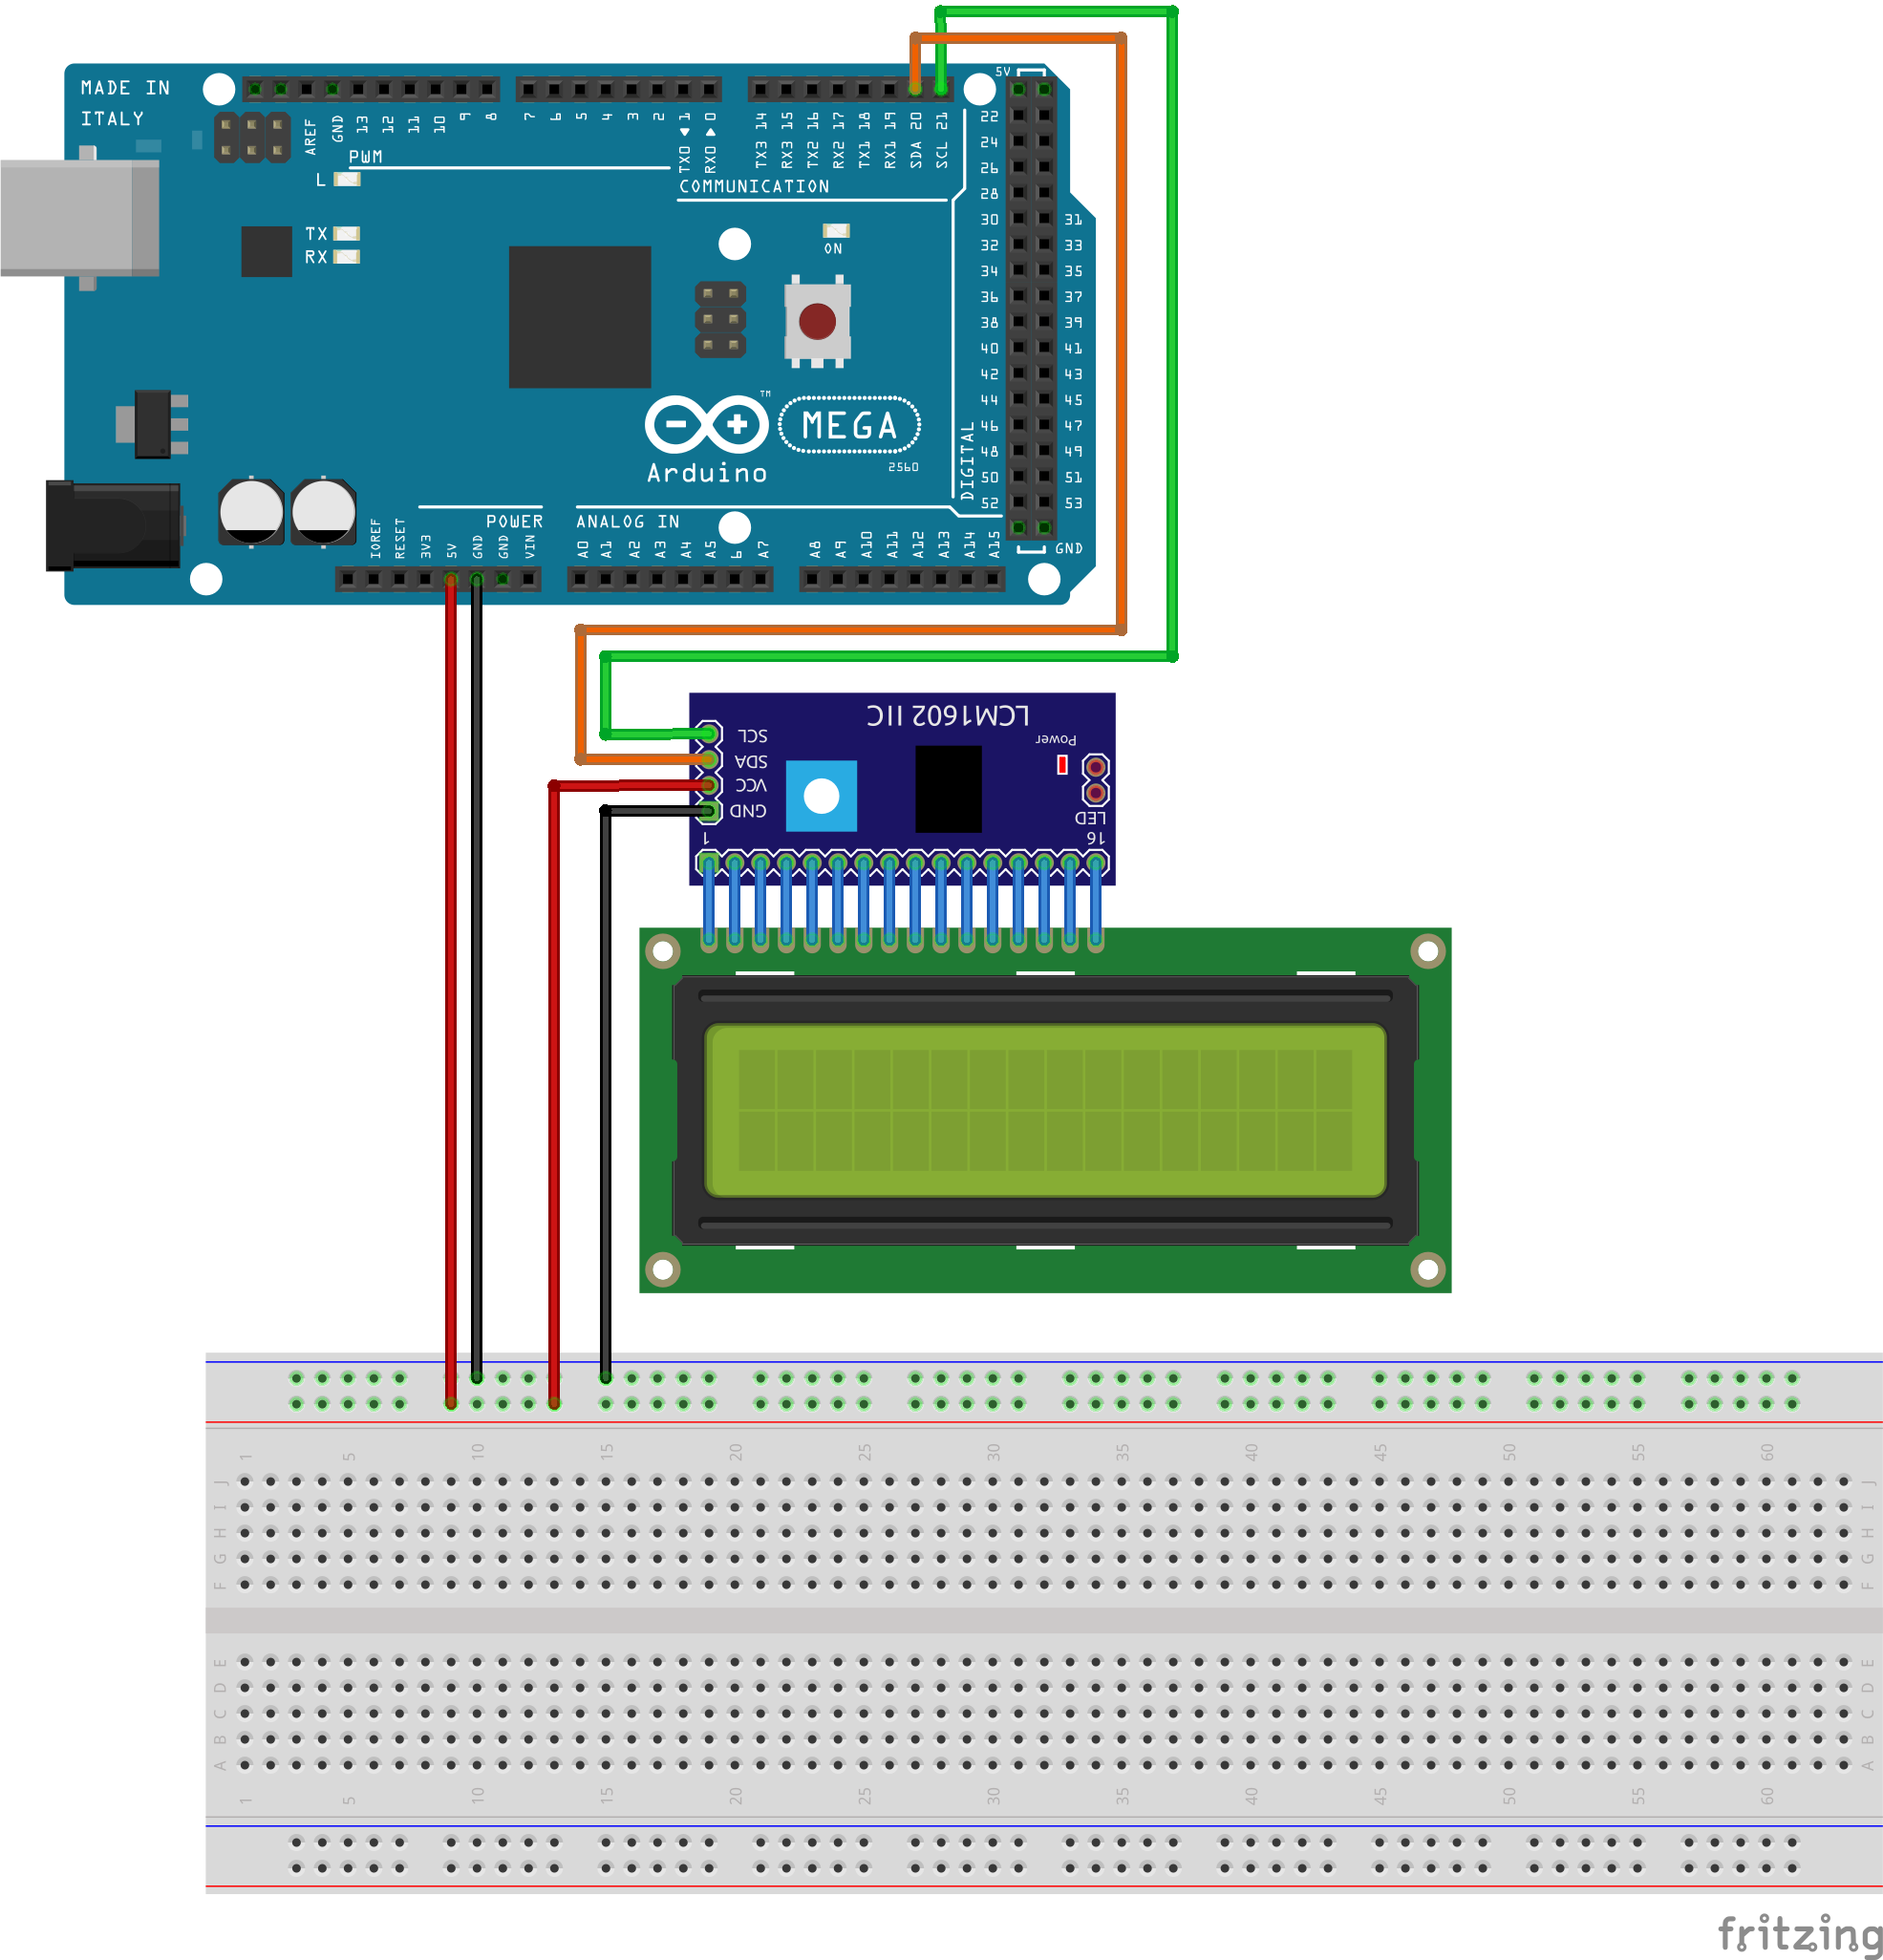
\includegraphics[width=12cm]{schematics/lcd-00}
    \caption{\figureCaption}
    \label{fig:lcd-00}
  \end{figure}
}

\newcommand{\figureMusicBarFourFour}[1]{
  \begin{tikzpicture}
    \draw[thick] (0, 0.5) -- (8, 0.5) node[anchor=north west] {t};
    \foreach \x/\n in {0/1, 8/2} {
      \draw (\x, 0) -- (\x, 1)  -- (\x, 1) node[midway, above] {\n};
    };

    \foreach \x in {0, 2, ..., 6} {
      \draw (\x, 0) -- (\x, 0.5) node[pos=0.25, right] {$ \frac{1}{4} $};
    };
  \end{tikzpicture}
}

\newcommand{\figureMusicBarFourFourWithFrequencies}[1]{
  \begin{tikzpicture}
    \draw[thick] (0, 0.5) -- (8, 0.5) node[anchor=north west] {t};
    \foreach \x/\n in {0/1, 8/2} {
      \draw (\x, 0) -- (\x, 1) -- (\x, 1) node[midway, above] {\n};
    };

    \foreach \x in {0, 2, ..., 6} {
      \draw (\x, 0) -- (\x, 0.5) node[pos=0.25, right] {$ \frac{1}{4} $};
    };

    \foreach \x/\freq in {0/50, 2/50, 4/50, 6/100} {
      \draw (\x, 0) -- (\x, 0.5) node[pos=1.5, right] {\freq Hz};
    };
  \end{tikzpicture}
}

\newcommand{\figureMusicSixBars}[1]{
  \begin{tikzpicture}
    \draw[thick, ->] (0, 0.5) -- (12, 0.5) node[anchor=north west] {t};
    \foreach \x/\n in {0/1, 2/2, 4/3, 6/4, 8/5, 10/6} {
      \draw (\x, 0) -- (\x, 1) -- (\x, 1) node[midway, above] {\n};
    };
    \label{fig:music-six-bar}
  \end{tikzpicture}
}

\newcommand{\figureMusicSixBarsFourFour}[1]{
  \begin{tikzpicture}
    \draw[thick, ->] (0, 0.5) -- (11, 0.5) node[anchor=north west] {t};
    \foreach \x/\n in {0/1, 2/2, 4/3, 6/4, 8/5, 10/6} {
      \draw (\x, 0) -- (\x, 1) -- (\x, 1) node[midway, above] {\n};
    };

    \foreach \x/\n in {0, 0.5, ..., 10} {
      \draw (\x, 0) -- (\x, 0.5);
    };
  \end{tikzpicture}
}

\newcommand{\figureMusicTripletExample}[1]{
  \def\lang{\detokenize{#1}}
  \def\langRu{\detokenize{ru}}
  \def\langEn{\detokenize{en}}
  \def\figureCaption{XXX: No translation.}
  \ifx \lang\langRu
  \def\figureCaption{
    Часть песни ``Hey You'' под авторством Pink Floyd.  Составлено на основе
    партитуры от Sam Anderson, опубликованной на Musescore:
    \url{https://musescore.com/user/33543481/scores/8040807}.
  }
  \fi
  \ifx \lang\langEn
  \def\figureCaption{
    A part of ``Hey You'' song by Pink Floyd.  Based on the music sheet by
    Sam Anderson, published on Musescore:
    \url{https://musescore.com/user/33543481/scores/8040807}
  }
  \fi
  \begin{figure}[ht]
    \centering
    \begin{lilypond}
      <<
      \new Staff {
        \relative g' {
          \tempo 4 = 112
          \numericTimeSignature
          \time 4/4
          \tuplet 3/2 {a4 b c} b8 a4 g8
        }
      }
      \new Staff {
        \clef "bass"
        \relative f {
          \numericTimeSignature
          \time 4/4
          d2 d2
        }
      }
      >>
      \layout {
        indent = 0\mm
        line-width = 100\mm
        ragged-last = ##t
      }
    \end{lilypond}
    \caption{\figureCaption}
    \label{fig:music-triplet-example}
  \end{figure}
}

\newcommand{\figureMusicTwinkleTwinkleLittleStar}[1]{
  \def\lang{\detokenize{#1}}
  \def\langRu{\detokenize{ru}}
  \def\langEn{\detokenize{en}}
  \def\figureCaption{XXX: No translation.}
  \ifx \lang\langRu
  \def\figureCaption{
    Мелодия ``Twinkle, Twinkle, Little Star''.
  }
  \fi
  \ifx \lang\langEn
  \def\figureCaption{
    ``Twinkle, Twinkle, Little Star'' melody.
  }
  \fi
  \begin{figure}[ht]
    \centering
    \begin{lilypond}
      \relative c' {
        \numericTimeSignature
        \time 4/4
        c4 c g' g
        a a g2
        f4 f e e
        d d c2
        g'4 g f f
        e e d2
        g4 g f f
        e e d2
        c4 c g' g
        a a g2
        f4 f e e
        d d c2
      }
      \layout {
        indent = 0\mm
        line-width = 100\mm
        ragged-last = ##t
      }
    \end{lilypond}
    \caption{\figureCaption}
    \label{fig:sound-fig-3}
  \end{figure}
}

\newcommand{\figureMusicWeWillRockYouSimplified}[1]{
  \def\lang{\detokenize{#1}}
  \def\langRu{\detokenize{ru}}
  \def\langEn{en}
  \def\figureCaption{XXX: No translation.}
  \ifx \lang\langRu
  \def\figureHzUnit{Гц}
  \def\figureCaption{
    Ритм мелодии ``We Will Rock You'' группы Queen (упрощенная версия.)
  }
  \fi
  \if \lang\langEn
  \def\figureHzUnit{Hz}
  \def\figureCaption{
    The rhythm of the melody ``We Will Rock You'' by Queen (simplified
    version.)
  }
  \fi
  \begin{figure}[ht]
    \centering
    \begin{tikzpicture}
      \draw[thick] (0, 0.5) -- (8, 0.5) node[anchor=north west] {t};
      \foreach \x/\n in {0/1, 8/2} {
        \draw (\x, 0) -- (\x, 1) -- (\x, 1) node[midway, above] {\n};
      };

      \foreach \x in {0, 2} {
        \draw (\x, 0) -- (\x, 0.5) node[pos=0.25, right] {$ \frac{1}{4} $};
      };

      \draw (4, 0) -- (4, 0.5) node[pos=0.25, right] {$ \frac{1}{2} $};

      \foreach \x/\freq in {0/50, 2/50} {
        \draw (\x, 0) -- (\x, 0.5) node[pos=1.5, right] {\freq \figureHzUnit};
      };
      \draw (4, 0) -- (4, 0.5) node[pos=1.5, right] {100 \figureHzUnit};
    \end{tikzpicture}
    \caption{\figureCaption}
    \label{fig:queen-we-will-rock-you-rhythm-1}
  \end{figure}
}

\newcommand{\figureProtocolClassification}[1]{
  \def\lang{\detokenize{#1}}
  \def\langRu{\detokenize{ru}}
  \def\langEn{\detokenize{en}}
  \def\figureCaption{XXX: No translation.}
  \def\figureDataTransfer{XXX: No translation.}
  \def\figureParallel{XXX: No translation.}
  \def\figureSerial{XXX: No translation.}
  \ifx \lang\langRu
  \def\figureCaption{
    Классификация методов передачи данных.
  }
  \def\figureDataTransfer{Передача данных}
  \def\figureParallel{Параллельная}
  \def\figureSerial{Последовательная}
  \fi
  \ifx \lang\langEn
  \def\figureCaption{
    Classification of data transferring methods.
  }
  \def\figureDataTransfer{Data transfer}
  \def\figureParallel{Parallel}
  \def\figureSerial{Serial}
  \fi
  \begin{figure}[H]
    \centering
    \begin{tikzpicture}[
        level distance=15mm,
        level 1/.style={sibling distance=30mm},
        level 2/.style={sibling distance=10mm},
        level 3/.style={sibling distance=15mm},
        every node/.style={rectangle,draw,inner sep=2pt},
      ]
      \node {\figureDataTransfer}
      child {node {\figureParallel}
        child {node {LPT}}
      }
      child {node {\figureSerial}
        child {node {UART}
          child {node {RS-232}}
          child {node {RS-485}}
        }
        child {node {SPI}}
        child {node {I2C}}
      };
    \end{tikzpicture}
    \caption{\figureCaption}
    \label{fig:communication-data-transfer-categories}
  \end{figure}
}

\newcommand{\figurePWMGraph}[2]{
  \def\lang{\detokenize{#1}}
  \def\langRu{\detokenize{ru}}
  \def\langEn{\detokenize{en}}
  \def\figureCaption{XXX: No translation.}
  \def\figureUnit{$\mu\mbox{s}$}
  \ifx \lang\langRu
  \def\figureCaption{
    Графическое отображение процесса генерации ШИМ-сигнала.
  }
  \def\figureUnit{мкс}
  \fi
  \ifx \lang\langEn
  \def\figureCaption{
    A graphical representation of the PWM signal generation.
  }
  \def\figureUnit{$\mu\mbox{s}$}
  \fi
  \begin{figure}[ht]
    \begin{tikzpicture}
      \draw[thick, ->] (0, 0) -- (12, 0) node[anchor=north west] {t};
      \draw[thick, ->] (0, 0) -- (0,  7) node[anchor=south west] {V};
      \draw[lightgray] (0, 0) grid (10, 6);
      \foreach \x in {0, 2, ..., 8} {
        \draw[ultra thick, teal] (\x, 6) -- (\x + 1, 6);
        \draw[ultra thick, teal] (\x + 1, 6) -- (\x + 1, 1);
        \draw[ultra thick, teal] (\x + 1, 1) -- (\x + 2, 1);
        \draw[ultra thick, teal] (\x + 2, 1) -- (\x + 2, 6);
      }
      \draw[ultra thick, teal, ->] (10, 6) -- (12, 6);
      \draw[orange] (10, 6) node[anchor=north west] {port=?};
      \draw[orange] (0, 6) node[anchor=north west] {d1};
      \draw[orange] (1, 6) node[anchor=north west] {d2};
      \draw[thick, orange] (0,  0) -- (0,   -2);
      \draw[thick, orange] (2,  1) -- (2,   -1);
      \draw[thick, orange] (10, 1) -- (10,  -2);
      \draw[thick, orange, <->] (0, -0.5) -- (2,  -0.5)  node[midway, below] {T=1000 \figureUnit};
      \draw[thick, orange, <->] (0, -1.5) -- (10,  -1.5) node[midway, below] {t=?};
    \end{tikzpicture}
    \caption{\figureCaption}
    \label{fig:pwm-graph}
  \end{figure}
}

\newcommand{\figureSerialPortDiagram}[1]{
  \def\lang{\detokenize{#1}}
  \def\langRu{\detokenize{ru}}
  \def\langEn{\detokenize{en}}
  \def\figureCaption{XXX: No translation.}
  \ifx \lang\langRu
  \def\figureCaption{
    Передача символа 'A' (код 65 в таблице ASCII, соответствет двоичному коду
    \texttt{01000001}) по последовательному порту.
  }
  \fi
  \ifx \lang\langEn
  \def\figureCaption{
    Transferring of 'A' symbol (code point 65 in the ASCII table, represented by
    the binary code \texttt{01000001} through a serial port.
  }
  \fi
  \begin{figure}[ht]
    \begin{tikzpicture}
      \draw[lightgray] (0, 0) grid (12, 4);
      \draw[lightgray, thick, ->] (0, 0) -- (13, 0) node[anchor=north west] {t};
      \draw[lightgray, thick, ->] (0, 0) -- (0,  5) node[anchor=south west] {V};
      \draw[ultra thick, black] (0,  2) -- (2,   2)
      %% 0 (start bit)
      -- (2,   1) -- (3,   1)
      %% 0
      -- (4,   1)
      %% 1
      -- (4,   2) -- (5,   2)
      %% 0 x 5
      -- (5,   1) -- (10,   1)
      %% 1
      -- (10,   2)
      -- (11,   2)
      %% 1 (stop bits)
      -- (12,   2);
      %% Draw digits.
      \draw[black]
      (0,  1) node[anchor=north west] {1}
      (1,  1) node[anchor=north west] {1}
      (2,  1) node[anchor=north west] {0}
      (3,  1) node[anchor=north west] {0}
      (4,  1) node[anchor=north west] {1}
      (5,  1) node[anchor=north west] {0}
      (6,  1) node[anchor=north west] {0}
      (7,  1) node[anchor=north west] {0}
      (8,  1) node[anchor=north west] {0}
      (9,  1) node[anchor=north west] {0}
      (10, 1) node[anchor=north west] {1}
      (11, 1) node[anchor=north west] {1};
      %% Draw comments.
      \draw[black]
      (2,  3) node[anchor=north west, text width=1cm] {start bit}
      (11, 3) node[anchor=north west, text width=1cm] {stop bit};
      %% Draw bits.
      \draw[black]
      (3,  3) node[anchor=north west] {D0}
      (4,  3) node[anchor=north west] {D1}
      (5,  3) node[anchor=north west] {D2}
      (6,  3) node[anchor=north west] {D3}
      (7,  3) node[anchor=north west] {D4}
      (8,  3) node[anchor=north west] {D5}
      (9,  3) node[anchor=north west] {D6}
      (10, 3) node[anchor=north west] {D7};
      \foreach \x in {3.5, 4.5, 5.5, 6.5, 7.5, 8.5, 9.5, 10.5} {
        \node at (\x, 1.5)[circle,fill,inner sep=1.5pt]{};
      };
      \draw[black, dotted] (3.5, 1.5) -- (3.5, -1);
      \draw[black, dotted] (4.5, 1.5) -- (4.5, -1);
      \draw[<->, black]
      (3.5, -1) node[anchor=north west, text width=1cm] {$T$}
      -- (4.5, -1);
    \end{tikzpicture}
    \caption{\figureCaption}
    \label{fig:communication-serial-port-diagram}
  \end{figure}
}

\newcommand{\figureSmallLCD}[1]{
  \def\lang{\detokenize{#1}}
  \def\langRu{\detokenize{ru}}
  \def\langEn{\detokenize{en}}
  \def\figureCaption{XXX: No translation.}
  \ifx \lang\langRu
  \def\figureCaption{
    Схематическое изображение внешнего вида ЖК-дисплея 16x2 (источник
    изображения: набор электронных компонентов программы Fritzing.)
  }
  \fi
  \ifx \lang\langEn
  \def\figureCaption{
    A schematic representation of an 16x2 LCD (source of the image:
    Fritzing electronic components library.)
  }
  \fi
  \begin{figure}[h]
    \centering
    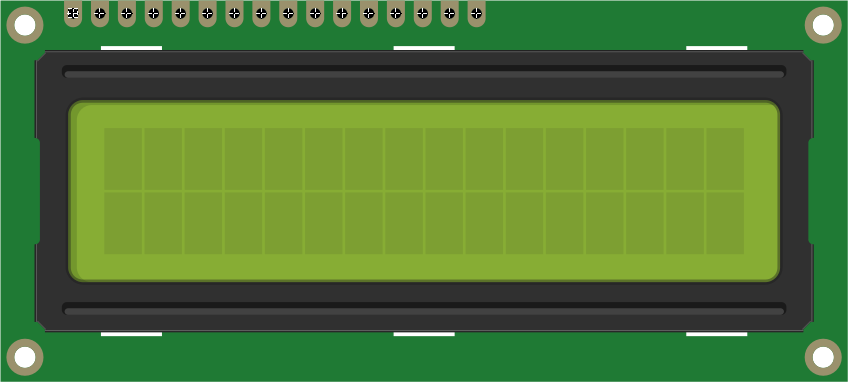
\includegraphics[width=10cm]{lcd-16x2}
    \caption{\figureCaption}
    \label{fig:lcd-16x2}
  \end{figure}
}

\newcommand{\figureSmallLCDShematics}[1]{
  \def\lang{\detokenize{#1}}
  \def\langRu{\detokenize{ru}}
  \def\langEn{\detokenize{en}}
  \def\figureCaption{XXX: No translation.}
  \ifx \lang\langRu
  \def\figureCaption{
    Схематическое изображение дисплея 16x2 (16 столбцов, 2 строки.)
  }
  \fi
  \ifx \lang\langEn
  \def\figureCaption{
    A schematic representation of an 16x2 LCD (16 columns, 2 rows.)
  }
  \fi
  \begin{figure}[ht]
    \centering
    \begin{tikzpicture}
      \draw[gray, step=0.5] (0, 0) grid (8, 1);
      \foreach [count=\i from 0] \x in {0.0, 0.5, 1.0, ..., 7.5} {
        \draw (\x, 1.5) node[anchor=north west] {\i};
      }
      \foreach [count=\i from 0] \y in {0.5, 0.0} {
        \draw (-0.5, \y) node[anchor=south west] {\i};
      }
    \end{tikzpicture}
    \caption{\figureCaption}
    \label{fig:lcd-16x2-schematics}
  \end{figure}
}

\newcommand{\figureSoundGraph}[1]{
  \begin{figure}[H]
    \begin{tikzpicture}
      \draw[thick, ->] (0, 0) -- (12, 0) node[anchor=north west] {t};
      \draw[thick, ->] (0, 0) -- (0,  7) node[anchor=south west] {V};
      \draw[lightgray] (0, 0) grid (10, 6);
      \foreach \x in {0, 2, ..., 8} {
        \draw[ultra thick, teal] (\x, 6) -- (\x + 1, 6);
        \draw[ultra thick, teal] (\x + 1, 6) -- (\x + 1, 1);
        \draw[ultra thick, teal] (\x + 1, 1) -- (\x + 2, 1);
        \draw[ultra thick, teal] (\x + 2, 1) -- (\x + 2, 6);
      }
      \draw[ultra thick, teal, ->] (10, 6) -- (12, 6);
      \draw[orange] (10, 6) node[anchor=north west, red] {port=?};
      \draw[orange] (0, 6) node[anchor=north west, red] {d};
      \draw[orange] (1, 6) node[anchor=north west, red] {d};
      \draw[thick, orange] (0,  0) -- (0,   -2);
      \draw[thick, orange] (2,  1) -- (2,   -1);
      \draw[thick, orange] (10, 1) -- (10,  -2);
      \draw[thick, orange, <->] (0, -0.5)
      -- (2,  -0.5) node[midway, below, red] {$\mbox{T} = \frac{1}{f}$};
      \draw[thick, orange, <->] (0, -1.5)
      -- (10,  -1.5) node[midway, below, red] {t=?};
    \end{tikzpicture}
    \caption{#1}
    \label{fig:sound-graph}
  \end{figure}
}

\newcommand{\tableCommunicationSerialPorts}[1]{
  \def\lang{\detokenize{#1}}
  \def\langRu{\detokenize{ru}}
  \def\langEn{\detokenize{en}}
  \def\tableFirstColumn{XXX: No translation.}
  \def\tableSecondColumn{XXX: No translation.}
  \ifx \lang\langRu
  \def\tableFirstColumn{Плата}
  \def\tableSecondColumn{Цифровые порты}
  \def\tableCaption{
    Последовательные порты на Arduino.
  }
  \fi
  \ifx \lang\langEn
  \def\tableFirstColumn{Board}
  \def\tableSecondColumn{Digital ports}
  \def\tableCaption{
    Serial ports on Arduino.
  }
  \fi

  \begin{table}[h]
    \centering
    \begin{tabular}{|m{9em}|m{3.5em}|m{3.5em}|m{3.5em}|m{3.5em}|m{3.5em}|}
      \hline
      \multirow{2}{2em}{\textbf{\tableFirstColumn}}
      & \multicolumn{5}{c|}{\textbf{\tableSecondColumn}} \\
      \cline{2-6}
      & \textbf{Serial}
      & \textbf{Serial1}
      & \textbf{Serial2}
      & \textbf{Serial3}
      & \textbf{Serial4} \\
      \hline
      UNO R3, UNO R3 SMD Mini
      & 0(RX), 1(TX) &                  &                  &                  &                  \\
      \hline
      Nano (classic)
      & 0(RX), 1(TX) &                  &                  &                  &                  \\
      \hline
      UNO R4 Minima, UNO R4 WiFi
      &              & 0(RX0), 1(TX0)   &                  &                  &                  \\
      \hline
      Leonardo, Micro, Yún Rev2
      &              & 0(RX), 1(TX)     &                  &                  &                  \\
      \hline
      Uno WiFi Rev.2
      &              & 0(RX), 1(TX)     &                  &                  &                  \\
      \hline
      MKR boards
      &              & 13(RX), 14(TX)   &                  &                  &                  \\
      \hline
      Zero
      &              & 0(RX), 1(TX)     &                  &                  &                  \\
      \hline
      GIGA R1 WiFi
      &              & 0(RX), 1(TX)     & 19(RX1), 18(TX1) & 17(RX2), 16(TX2) & 15(RX3), 14(TX3) \\
      \hline
      Due
      & 0(RX), 1(TX) & 19(RX1), 18(TX1) & 17(RX2), 16(TX2) & 15(RX3), 14(TX3) &                  \\
      \hline
      Mega 2560 Rev3
      & 0(RX), 1(TX) & 19(RX1), 18(TX1) & 17(RX2), 16(TX2) & 15(RX3), 14(TX3) &                  \\
      \hline
      Nano 33 IoT
      &              & 0(RX0), 1(TX0)   &                  &                  &                  \\
      \hline
      Nano RP2040 Connect
      &              & 0(RX0), 1(TX0)   &                  &                  &                  \\
      \hline
      Nano BLE / BLE Sense
      &              & 0(RX0), 1(TX0)   &                  &                  & \\
      \hline
    \end{tabular}
    \caption{\tableCaption}
    \label{table:serial-ports--pins}
  \end{table}
}

\newcommand{\tableMusicNoteLength}[1]{
  \def\lang{\detokenize{#1}}
  \def\langRu{\detokenize{ru}}
  \def\langEn{\detokenize{en}}
  \def\tableFirstColumn{XXX: No translation.}
  \def\tableSecondColumn{XXX: No translation.}
  \def\tableThirdColumn{XXX: No translation.}
  \def\tableCaption{XXX: No translation.}
  \def\tableWholeNote{XXX: No translation.}
  \def\tableHalfNote{XXX: No translation.}
  \def\tableQuarterNote{XXX: No translation.}
  \def\tableEighthNote{XXX: No translation.}
  \def\tableSixteenthNote{XXX: No translation.}
  \ifx \lang\langRu
  \def\tableFirstColumn{Начертание}
  \def\tableSecondColumn{Длительность}
  \def\tableThirdColumn{Название}
  \def\tableCaption{
    Некоторые возможные длительности нот.
  }
  \def\tableWholeNote{Целая}
  \def\tableHalfNote{Половина}
  \def\tableQuarterNote{Четверть}
  \def\tableEighthNote{Восьмая}
  \def\tableSixteenthNote{Шестнадцатая}
  \fi
  \ifx \lang\langEn
  \def\tableFirstColumn{Symbol}
  \def\tableSecondColumn{Length}
  \def\tableThirdColumn{Title}
  \def\tableCaption{
    Some of the possible lengths of the musical sounds (notes.)
  }
  \def\tableWholeNote{Whole note}
  \def\tableHalfNote{Half-note}
  \def\tableQuarterNote{Quarter-note}
  \def\tableEighthNote{Eighth-note}
  \def\tableSixteenthNote{Sixteenth-note}
  \fi

  \begin{table}[ht]
    \centering
    \def\arraystretch{2.5}%
    \begin{tabular}{|m{3cm}|m{4cm}|m{3.5cm}|}
      \hline
      \textbf{\tableFirstColumn}
      & \textbf{\tableSecondColumn}
      & \textbf{\tableThirdColumn} \\
      \hline
      {\Large \wholeNote} & {\Large $\frac{1}{1}$} & \tableWholeNote \\[2ex]
      \hline
      {\Large \halfNote}      & {\Large $\frac{1}{2}$}  & \tableHalfNote \\[2ex]
      \hline
      {\Large \quarterNote}   & {\Large $\frac{1}{4}$}  & \tableQuarterNote \\[2ex]
      \hline
      {\Large \eighthNote}    & {\Large $\frac{1}{8}$}  & \tableEighthNote \\[2ex]
      \hline
      {\Large \sixteenthNote} & {\Large $\frac{1}{16}$} & \tableSixteenthNote \\[2ex]
      \hline
    \end{tabular}
    \caption{\tableCaption}
    \label{table:music-notes-legths}
  \end{table}
}

\newcommand{\tableMusicOctaveExample}[1]{
  \def\lang{\detokenize{#1}}
  \def\langRu{\detokenize{ru}}
  \def\langEn{\detokenize{en}}
  \def\tableFirstColumn{XXX: No translation.}
  \def\tableSecondColumn{XXX: No translation.}
  \def\tableThirdColumn{XXX: No translation.}
  \def\tableFourthColumn{XXX: No translation.}
  \def\tableCaption{XXX: No translation.}
  \ifx \lang\langRu
  \def\tableFirstColumn{
    № октавы
  }
  \def\tableSecondColumn{
    Слоговое обозначение
  }
  \def\tableThirdColumn{
    Научное обознечение
  }
  \def\tableFourthColumn{
    Частота (Гц)
  }
  \def\tableCaption{
    Пример двух октав.
  }
  \fi
  \ifx \lang\langEn
  \def\tableFirstColumn{
    Octave
  }
  \def\tableSecondColumn{
    Syllable notation
  }
  \def\tableThirdColumn{
    Scientific notation
  }
  \def\tableFourthColumn{
    Frequency (Hz)
  }
  \def\tableCaption{
    An example of two octaves.
  }
  \fi
  \begin{table}[ht]
    \centering
    \begin{tabular}{|p{1.5cm}|p{3cm}|p{3cm}|p{2.5cm}|}
      \hline
      \textbf{\tableFirstColumn}
      & \textbf{\tableSecondColumn}
      & \textbf{\tableThirdColumn}
      & \textbf{\tableFourthColumn} \\
      \hline
      \multirow{7}{*}{0}
      \musicnote{#1}{0}{C}{16.352}
      \cline{2-4}
      \musicnote{#1}{0}{D}{18.354}
      \cline{2-4}
      \musicnote{#1}{0}{E}{20.602}
      \cline{2-4}
      \musicnote{#1}{0}{F}{21.827}
      \cline{2-4}
      \musicnote{#1}{0}{G}{24.500}
      \cline{2-4}
      \musicnote{#1}{0}{A}{27.500}
      \cline{2-4}
      \musicnote{#1}{0}{B}{30.868}
      \hline

      \multirow{7}{*}{4}
      \musicnote{#1}{4}{C}{261.630}
      \cline{2-4}
      \musicnote{#1}{4}{D}{293.660}
      \cline{2-4}
      \musicnote{#1}{4}{E}{329.630}
      \cline{2-4}
      \musicnote{#1}{4}{F}{349.230}
      \cline{2-4}
      \musicnote{#1}{4}{G}{392.000}
      \cline{2-4}
      \musicnote{#1}{4}{A}{440.000}
      \cline{2-4}
      \musicnote{#1}{4}{B}{493.880}
      \hline
    \end{tabular}
    \caption{\tableCaption}
    \label{table:fourth-octave}
  \end{table}
}

\newcommand{\tableMusicTwinkleTwinkleLittleStar}[1]{
  \def\lang{\detokenize{#1}}
  \def\langRu{\detokenize{ru}}
  \def\langEn{\detokenize{en}}
  \def\tableFirstColumn{XXX: No translation.}
  \def\tableSecondColumn{XXX: No translation.}
  \ifx \lang\langRu
  \def\tableFirstColumn{№ такта}
  \def\tableSecondColumn{Ноты}
  \def\tableCaption{
    Ноты мелодии ``Twinkle, Twinkle, Little Star''.
  }
  \fi
  \ifx \lang\langEn
  \def\tableFirstColumn{Bar number}
  \def\tableSecondColumn{Notes}
  \def\tableCaption{
    Notes of ``Twinkle, Twinkle, Little Star'' melody.
  }
  \fi

  \begin{table}[ht]
    \centering
    \def\arraystretch{2.5}%
    \begin{tabular}{|p{2cm}|p{2cm}|p{2cm}|p{2cm}|p{2cm}|}
      \hline
      \textbf{\tableFirstColumn}
      & \multicolumn{4}{c|}{\textbf{\tableSecondColumn}} \\
      \hline
      0
      & C4 ($\frac{1}{4}$)
      & C4 ($\frac{1}{4}$)
      & G4 ($\frac{1}{4}$)
      & G4 ($\frac{1}{4}$) \\
      \hline
      1
      & A4 ($\frac{1}{4}$)
      & A4 ($\frac{1}{4}$)
      & G4 ($\frac{1}{2}$)
      & \\
      \hline
      2
      & F4 ($\frac{1}{4}$)
      & F4 ($\frac{1}{4}$)
      & E4 ($\frac{1}{4}$)
      & E4 ($\frac{1}{4}$) \\
      \hline
      3
      & D4 ($\frac{1}{4}$)
      & D4 ($\frac{1}{4}$)
      & C4 ($\frac{1}{2}$)
      & \\
      \hline
      4
      & G4 ($\frac{1}{4}$)
      & G4 ($\frac{1}{4}$)
      & F4 ($\frac{1}{4}$)
      & F4 ($\frac{1}{4}$) \\
      \hline
      5
      & E4 ($\frac{1}{4}$)
      & E4 ($\frac{1}{4}$)
      & D4 ($\frac{1}{2}$)
      & \\
      \hline
      6
      & G4 ($\frac{1}{4}$)
      & G4 ($\frac{1}{4}$)
      & F4 ($\frac{1}{4}$)
      & F4 ($\frac{1}{4}$) \\
      \hline
      7
      & E4 ($\frac{1}{4}$)
      & E4 ($\frac{1}{4}$)
      & D4 ($\frac{1}{2}$)
      & \\
      \hline
      8
      & C4 ($\frac{1}{4}$)
      & C4 ($\frac{1}{4}$)
      & G4 ($\frac{1}{4}$)
      & G4 ($\frac{1}{4}$) \\
      \hline
      9
      & A4 ($\frac{1}{4}$)
      & A4 ($\frac{1}{4}$)
      & G4 ($\frac{1}{2}$)
      & \\
      \hline
    \end{tabular}
    \caption{\tableCaption}
    \label{table:twinkle-twinkle-little-star-notes-lengths}
  \end{table}
}

\newcommand{\tableMusicTwinkleTwinkleLittleStarNotes}[1]{
  \def\lang{\detokenize{#1}}
  \def\langRu{\detokenize{ru}}
  \def\langEn{\detokenize{en}}
  \def\tableFirstColumn{XXX: No translation.}
  \def\tableSecondColumn{XXX: No translation.}
  \ifx \lang\langRu
  \def\tableFirstColumn{№ такта}
  \def\tableSecondColumn{Ноты}
  \def\tableCaption{
    Ноты мелодии ``Twinkle, Twinkle, Little Star'' (без длительностей.)
  }
  \fi
  \ifx \lang\langEn
  \def\tableFirstColumn{Bar number}
  \def\tableSecondColumn{Notes}
  \def\tableCaption{
    Notes of ``Twinkle, Twinkle, Little Star'' melody (without the lengths.)
  }
  \fi

  \begin{table}[H]
    \centering
    \begin{tabular}{|p{2cm}|p{2cm}|p{2cm}|p{2cm}|p{2cm}|}
      \hline
      \textbf{\tableFirstColumn}
      & \multicolumn{4}{|c|}{\tableSecondColumn} \\
      \hline
      0 & C4 & C4 & G4 & G4 \\
      \hline
      1 & A4 & A4 & G4 & \\
      \hline
      2 & F4 & F4 & E4 & E4 \\
      \hline
      3 & D4 & D4 & C4 & \\
      \hline
      4 & G4 & G4 & F4 & F4 \\
      \hline
      5 & E4 & E4 & D4 & \\
      \hline
      6 & G4 & G4 & F4 & F4 \\
      \hline
      7 & E4 & E4 & D4 & \\
      \hline
      8 & C4 & C4 & G4 & G4 \\
      \hline
      9 & A4 & A4 & G4 & \\
      \hline
    \end{tabular}
    \caption{\tableCaption}
    \label{table:twinkle-twinkle-little-star-notes}
  \end{table}
}

\newcommand{\tableIICPorts}[1]{
  \def\lang{\detokenize{#1}}
  \def\langRu{\detokenize{ru}}
  \def\langEn{\detokenize{en}}
  \def\tableFirstColumn{XXX: No translation.}
  \def\tableSecondColumn{XXX: No translation.}
  \def\tableCaption{XXX: No translation.}
  \ifx \lang\langRu
  \def\tableFirstColumn{
    Плата
  }
  \def\tableSecondColumn{
    Порты I2C
  }
  \def\tableCaption{
    I2C-порты на разных платформах Arduino.
  }
  \fi
  \ifx \lang\langEn
  \def\tableFirstColumn{
    Board
  }
  \def\tableSecondColumn{
    I2C Ports
  }
  \def\tableCaption{
    I2C ports on different Arduino boards.
  }
  \fi
  \begin{table}[h]
    \centering
    \begin{tabular}{ | c | c | c | }
      \hline
      \multirow{2}{8em}{\textbf{\tableFirstColumn}}
      & \multicolumn{2}{c|}{\textbf{\tableSecondColumn}} \\
      \cline{2-3}
      & \textbf{SDA} & \textbf{SCL} \\
      \hline
      Nano & A4 & A5 \\
      \hline
      UNO R3 & A4 & A5 \\
      \hline
      Leonardo & D2 & D3 \\
      \hline
      Mega 2560 Rev3 & D20 & D21 \\
      \hline
      Due & D20 & D21 \\
      \hline
    \end{tabular}
    \caption{\tableCaption}
    \label{table:i2c-pins}
  \end{table}
}

\newcommand{\tableInterrupts}[1]{
  \def\lang{\detokenize{#1}}
  \def\langRu{\detokenize{ru}}
  \def\langEn{\detokenize{en}}
  \def\tableCaption{XXX: No translation.}
  \def\tableFirstColumn{XXX: No translation.}
  \ifx \lang\langRu
  \def\tableFirstColumn{Плата}
  \def\tableCaption{
    Номера прерываний и связанных с ними цифровых портов.
  }
  \fi
  \ifx \lang\langEn
  \def\tableFirstColumn{Board}
  \def\tableCaption{
    Interrupt numbers and digital ports related to them.
  }
  \fi
  \begin{table}[ht]
    \centering
    \def\arraystretch{1.5}%
    \begin{tabular}{|m{2.5cm}|m{1cm}|m{1cm}|m{1cm}|m{1cm}|m{1cm}|m{1cm}|}
      \hline
      \textbf{\tableFirstColumn}
      & \textbf{\texttt{int.0}}
      & \textbf{\texttt{int.1}}
      & \textbf{\texttt{int.2}}
      & \textbf{\texttt{int.3}}
      & \textbf{\texttt{int.4}}
      & \textbf{\texttt{int.5}}\\
      \hline
      Arduino Uno  & 2 & 3 &    &    &    &   \\[1.5ex]
      \hline
      Arduino Mega & 2 & 3 & 21 & 20 & 19 & 18\\[1.5ex]
      \hline
    \end{tabular}
    \caption{\tableCaption}
    \label{table:interrupts-table}
  \end{table}
}

\newcommand{\tableLCM}[1]{
  \def\lang{\detokenize{#1}}
  \def\langRu{\detokenize{ru}}
  \def\langEn{\detokenize{en}}
  \def\tableFirstColumn{XXX: No translation.}
  \def\tableSecondColumn{XXX: No translation.}
  \def\tableThirdColumn{XXX: No translation.}
  \def\tableCaption{XXX: No translation.}
  \ifx \lang\langRu
  \def\tableFirstColumn{
    Подключение пинов
  }
  \def\tableSecondColumn{
    Конфигурация адреса
  }
  \def\tableThirdColumn{
    Адрес I2C
  }
  \def\tableCaption{
    Адресация модуля LCM1602-I2C.
  }
  \fi
  \ifx \lang\langEn
  \def\tableFirstColumn{
    Pin connections
  }
  \def\tableSecondColumn{
    Address configuration
  }
  \def\tableThirdColumn{
    I2C address
  }
  \def\tableCaption{
    Address configuration on LCM1602-I2C module.
  }
  \fi
  \begin{table}[H]
    \centering
    \begin{tabular}{
        %% A2-A0
        | c | c | c
        %% A6-A0
        | c | c | c | c | c | c | c
        %% R/W
        | c
        %% Address
        | c
        | }
      \hline
      \multicolumn{3}{|c|}{\textbf{Подключение пинов}}
      & \multicolumn{8}{c|}{\textbf{Конфигурация адреса}}
      & \multirow{2}{2em}{\textbf{Адрес I2C}} \\
      \cline{1-11}
      \textbf{A2}
      & \textbf{A1}
      & \textbf{A0}
      & \textbf{A6}
      & \textbf{A5}
      & \textbf{A4}
      & \textbf{A3}
      & \textbf{A2}
      & \textbf{A1}
      & \textbf{A0}
      & \textbf{R/W}
      &   \\
      \hline
      $V_{SS}$ & $V_{SS}$ & $V_{SS}$ & 0 & 1 & 0 & 0 & 0 & 0 & 0 & -- & \texttt{0x20} \\
      \hline
      $V_{SS}$ & $V_{SS}$ & $V_{DD}$ & 0 & 1 & 0 & 0 & 0 & 0 & 1 & -- & \texttt{0x21} \\
      \hline
      $V_{SS}$ & $V_{DD}$ & $V_{SS}$ & 0 & 1 & 0 & 0 & 0 & 1 & 0 & -- & \texttt{0x22} \\
      \hline
      $V_{SS}$ & $V_{DD}$ & $V_{DD}$ & 0 & 1 & 0 & 0 & 0 & 1 & 1 & -- & \texttt{0x23} \\
      \hline
      $V_{DD}$ & $V_{SS}$ & $V_{SS}$ & 0 & 1 & 0 & 0 & 1 & 0 & 0 & -- & \texttt{0x24} \\
      \hline
      $V_{DD}$ & $V_{SS}$ & $V_{DD}$ & 0 & 1 & 0 & 0 & 1 & 0 & 1 & -- & \texttt{0x25} \\
      \hline
      $V_{DD}$ & $V_{DD}$ & $V_{SS}$ & 0 & 1 & 0 & 0 & 1 & 1 & 0 & -- & \texttt{0x26} \\
      \hline
      $V_{DD}$ & $V_{DD}$ & $V_{DD}$ & 0 & 1 & 0 & 0 & 1 & 1 & 1 & -- & \texttt{0x27} \\
      \hline
    \end{tabular}
    \caption{Адресация модуля LCM1602-I2C.}
    \label{table:i2c-lcm1602-addressing}
  \end{table}
}

\newcommand{\tableTwoDimensionalArray}[1]{
  \def\lang{\detokenize{#1}}
  \def\langRu{\detokenize{ru}}
  \def\langEn{\detokenize{en}}
  \def\tableFirstColumn{XXX: No translation.}
  \def\tableSecondColumn{XXX: No translation.}
  \def\tableCaption{XXX: No translation.}
  \ifx \lang\langRu
  \def\tableFirstColumn{
    № строки
  }
  \def\tableSecondColumn{
    № столбца
  }
  \def\tableCaption{
    Графическое отображение двумерного массива.
  }
  \fi
  \ifx \lang\langEn
  \def\tableFirstColumn{
    Row number
  }
  \def\tableSecondColumn{
    Column number
  }
  \def\tableCaption{
    Graphical representation of a two-dimensional array.
  }
  \fi
  \begin{table}[ht]
    \centering
    \begin{tabular}{r|l|l|l}
      \multicolumn{1}{l}{\tableFirstColumn}
      & \multicolumn{2}{l}{\tableSecondColumn}
      & \\
      \multicolumn{1}{l}{}         & \multicolumn{1}{l}{0} & \multicolumn{1}{l}{1} &   \\
      \cline{2-3}
      0                            & с4                    & 4                     &   \\
      \cline{2-3}
      1                            & с4                    & 4                     &   \\
      \cline{2-3}
      2                            & g4                    & 4                     &   \\
      \cline{2-3}
      3                            & g4                    & 4                     &   \\
      \cline{2-3}
      4                            & a4                    & 4                     &   \\
      \cline{2-3}
      5                            & a4                    & 4                     &   \\
      \cline{2-3}
      6                            & g4                    & 2                     &   \\
      \cline{2-3}
    \end{tabular}
    \caption{\tableCaption}
    \label{table:array-example-2}
  \end{table}
}


\counterwithin{listing}{section}
\renewcommand\listingscaption{Листинг}

\newgetenv[\REPRODUCIBILITY]{REPRODUCIBILITY}%
\newgetenv[\RANDOMSEED]{RANDOMSEED}

\ifdefstring{\REPRODUCIBILITY}{yes}{%
  \ifthenelse{\equal{\RANDOMSEED}{}}%
  {%
    \typeout{Setting the random seed to a fixed value.}%
    \pgfmathsetseed{\number42}%
  }{%
    \typeout{Setting the random seed to a \RANDOMSEED .}%
    \pgfmathsetseed{\number\RANDOMSEED}%
  }%
}{}

%%%%%%%%%%%%%%%%%%%%%%%%%%%%%%%%%%%%%%%%%%%%%%%%%%%%%%%%%%%%%%%%%%%%%%%%%%%%%%%%
\title{Автомато-программато-компарадио-кружок}
\author{Артём ``avp'' Попцов\\\href{https://memory-heap.org}{memory-heap.org}}
\input{version.tex}

\begin{document}

\maketitle

\tableofcontents

%%%%%%%%%%%%%%%%%%%%%%%%%%%%%%%%%%%%%%%%%%%%%%%%%%%%%%%%%%%%%%%%%%%%%%%%%%%%%%%%
\chapter*{Вступление}
\addcontentsline{toc}{chapter}{Вступление}

\subfile{sections/introduction.tex}

%%%%%%%%%%%%%%%%%%%%%%%%%%%%%%%%%%%%%%%%%%%%%%%%%%%%%%%%%%%%%%%%%%%%%%%%%%%%%%%%
\chapter{Основы электроники}

В первую очередь нам с вами надо рассмотреть базовые принципы того, как работает
электроника, чтобы впоследствии уметь собирать простые схемы.

Начнём с рассмотрения условий, которые необходимо выполнить, чтобы через
электрическую цепь шёл ток.

\subfile{sections/electronics-voltage}
\subfile{sections/electronics-circuits}
\subfile{sections/electronics-potential-difference}
\subfile{sections/electronics-resistance}
\subfile{sections/electronics-building-circuits}

%%%%%%%%%%%%%%%%%%%%%%%%%%%%%%%%%%%%%%%%%%%%%%%%%%%%%%%%%%%%%%%%%%%%%%%%%%%%%%%%
\chapter{Диалоги с компьютером}
\label{chapter:dialogues-with-computer}

\subfile{sections/dialogues-with-computer-title-image}
\subfile{sections/dialogues-with-computer-introduction}
\subfile{sections/dialogues-with-computer-arduino}
\subfile{sections/dialogues-with-computer-breadboard}
\subfile{sections/dialogues-with-computer-multimeter}

\newpage
\subfile{sections/dialogues-with-computer-arduino-ide}
\subfile{sections/dialogues-with-computer-algorithms}
\subfile{sections/dialogues-with-computer-program-structure}
\subfile{sections/dialogues-with-computer-memory}
\subfile{sections/dialogues-with-computer-control-flow}
\subfile{sections/dialogues-with-computer-wokwi}

%%%%%%%%%%%%%%%%%%%%%%%%%%%%%%%%%%%%%%%%%%%%%%%%%%%%%%%%%%%%%%%%%%%%%%%%%%%%%%%%
\chapter{Белый шум}

\subfile{sections/white-noise-introduction}
\subfile{sections/white-noise-signal-types}
\subfile{sections/white-noise-serial-port}
\subfile{sections/white-noise-analog-ports}
\subfile{sections/white-noise-adc}

%%%%%%%%%%%%%%%%%%%%%%%%%%%%%%%%%%%%%%%%%%%%%%%%%%%%%%%%%%%%%%%%%%%%%%%%%%%%%%%%
\chapter{Широтно-импульсная модуляция}
\label{chapter:pwm}

\subfile{sections/pwm-intro}
\subfile{sections/pwm-wavelength}
\subfile{sections/pwm-duty-cycle}
\subfile{sections/pwm-tasks}

%%%%%%%%%%%%%%%%%%%%%%%%%%%%%%%%%%%%%%%%%%%%%%%%%%%%%%%%%%%%%%%%%%%%%%%%%%%%%%%%
\chapter{Синтез музыки и технологии}

\subfile{sections/music-and-technology-synthesis-sound}
\subfile{sections/music-and-technology-synthesis-speaker}
\subfile{sections/music-and-technology-synthesis-rhythm}
\subfile{sections/music-and-technology-synthesis-harmony}
\subfile{sections/music-and-technology-synthesis-octave-system}
\subfile{sections/music-and-technology-synthesis-simple-melodies}
\subfile{sections/music-and-technology-synthesis-arrays}
\subfile{sections/music-and-technology-synthesis-two-dimensional-arrays}
\subfile{sections/music-and-technology-synthesis-staff}
\subfile{sections/music-and-technology-synthesis-rest}
\subfile{sections/music-and-technology-synthesis-dotted-notes}
\subfile{sections/music-and-technology-synthesis-triplet}
\subfile{sections/music-and-technology-synthesis-flats-and-sharps}
\subfile{sections/music-and-technology-synthesis-musical-scale}
\subfile{sections/music-and-technology-synthesis-bass-clef}
\subfile{sections/music-and-technology-synthesis-music-band}

%%%%%%%%%%%%%%%%%%%%%%%%%%%%%%%%%%%%%%%%%%%%%%%%%%%%%%%%%%%%%%%%%%%%%%%%%%%%%%%%
\chapter{Язык общения машин}
\subfile{sections/communication-intro}
\subfile{sections/communication-serial-port}
\subfile{sections/communication-i2c}

%%%%%%%%%%%%%%%%%%%%%%%%%%%%%%%%%%%%%%%%%%%%%%%%%%%%%%%%%%%%%%%%%%%%%%%%%%%%%%%%
\chapter{Разработка игр}
\label{chapter:game-dev}

\subfile{sections/game-dev-intro}
\subfile{sections/game-dev-lcd}
\subfile{sections/game-dev-genre-and-plot}
\subfile{sections/game-dev-player}
\subfile{sections/game-dev-buttons}
\subfile{sections/game-dev-game-map}
\subfile{sections/game-dev-sounds}
\subfile{sections/game-dev-graphics}
\subfile{sections/game-dev-animation}
\subfile{sections/game-dev-logic}
\subfile{sections/game-dev-structures}

%%%%%%%%%%%%%%%%%%%%%%%%%%%%%%%%%%%%%%%%%%%%%%%%%%%%%%%%%%%%%%%%%%%%%%%%%%%%%%%%
\chapter{Обработка прерываний}
\subfile{sections/interrupts-intro}
\subfile{sections/interrupts-types}
\subfile{sections/interrupts-hw-external}
\subfile{sections/interrupts-hw-internal}

%%%%%%%%%%%%%%%%%%%%%%%%%%%%%%%%%%%%%%%%%%%%%%%%%%%%%%%%%%%%%%%%%%%%%%%%%%%%%%%%
\addcontentsline{toc}{chapter}{Предметный указатель}
\printindex

%%%%%%%%%%%%%%%%%%%%%%%%%%%%%%%%%%%%%%%%%%%%%%%%%%%%%%%%%%%%%%%%%%%%%%%%%%%%%%%%
\addcontentsline{toc}{chapter}{Словарь терминов}
\printglossaries

%%%%%%%%%%%%%%%%%%%%%%%%%%%%%%%%%%%%%%%%%%%%%%%%%%%%%%%%%%%%%%%%%%%%%%%%%%%%%%%%
\addcontentsline{toc}{chapter}{Список примеров кода}
\renewcommand\listoflistingscaption{Список примеров кода}
\listoflistings

%%%%%%%%%%%%%%%%%%%%%%%%%%%%%%%%%%%%%%%%%%%%%%%%%%%%%%%%%%%%%%%%%%%%%%%%%%%%%%%%
\printbibliography[heading=bibintoc, title={Библиография}]

%%%%%%%%%%%%%%%%%%%%%%%%%%%%%%%%%%%%%%%%%%%%%%%%%%%%%%%%%%%%%%%%%%%%%%%%%%%%%%%%
\appendix

\subfile{sections/appendix-octaves}
\subfile{sections/appendix-prostokvashino-score}
\subfile{sections/appendix-twinkle-twinkle-little-star-01}
\subfile{sections/appendix-twinkle-twinkle-little-star-02}

\end{document}

